\documentclass[UTF8,11pt]{ctexart}
\usepackage[a4paper,margin=22mm]{geometry}
\usepackage{amsmath,amssymb,bm,graphicx,adjustbox,fvextra,longtable,array}
\xeCJKDeclareCharClass{CJK}{"2160 -> "217F, "2460 -> "249B, "2200 -> "22FF}
\newcommand{\fitmath}[1]{\begin{adjustbox}{max width=\linewidth}$\displaystyle #1$\end{adjustbox}}
\setlength{\parindent}{0pt}\setlength{\parskip}{.65em}\renewcommand{\arraystretch}{1.3}
\sloppy\allowdisplaybreaks
\begin{document}
\section*{2010 年计算机统考 408 · 真题及解析}
\subsection*{2010 年全国硕士研究生入学统一考试计算机科学与技术学科联考计算机学科专业基础综合试题}

\subsection*{一、单项选择题：第1\textasciitilde{}40 小题，每小题2 分，共80 分。下列每题给出的四个选项中，只有一个选项最符合试题要求。}

1. 若元素a、b、c、d、e、f 依次进栈，允许进栈、退栈操作交替进行，但不允许连续三次进行退栈操作，则不．可能得到的出栈序列是\_\_\_\_\_\_。


\begin{center}\begin{tabular}{>{\raggedright\arraybackslash}p{\dimexpr(\linewidth-8\tabcolsep)/4\relax}>{\raggedright\arraybackslash}p{\dimexpr(\linewidth-8\tabcolsep)/4\relax}>{\raggedright\arraybackslash}p{\dimexpr(\linewidth-8\tabcolsep)/4\relax}>{\raggedright\arraybackslash}p{\dimexpr(\linewidth-8\tabcolsep)/4\relax}}
\textbf{A.} d c e b f a & \textbf{B.} c b d a e f & \textbf{C.} b c a e f d & \textbf{D.} a f e d c b\\[.35em]\end{tabular}\end{center}

2. 某队列允许在其两端进行入队操作，但仅允许在一端进行出队操作。若元素a、b、c、d、e 依次入此队列后再进行出队操作，则不．可能得到的出队序列是\_\_\_\_\_\_。


\begin{center}\begin{tabular}{>{\raggedright\arraybackslash}p{\dimexpr(\linewidth-8\tabcolsep)/4\relax}>{\raggedright\arraybackslash}p{\dimexpr(\linewidth-8\tabcolsep)/4\relax}>{\raggedright\arraybackslash}p{\dimexpr(\linewidth-8\tabcolsep)/4\relax}>{\raggedright\arraybackslash}p{\dimexpr(\linewidth-8\tabcolsep)/4\relax}}
\textbf{A.} b a c d e & \textbf{B.} d b a c e & \textbf{C.} d b c a e & \textbf{D.} e c b a d\\[.35em]\end{tabular}\end{center}

3. 下列线索二叉树中（用虚线表示线索），符合后序线索树定义的是\_\_\_\_\_\_。


\begin{center}\begin{tabular}{>{\raggedright\arraybackslash}p{\dimexpr(\linewidth-8\tabcolsep)/4\relax}>{\raggedright\arraybackslash}p{\dimexpr(\linewidth-8\tabcolsep)/4\relax}>{\raggedright\arraybackslash}p{\dimexpr(\linewidth-8\tabcolsep)/4\relax}>{\raggedright\arraybackslash}p{\dimexpr(\linewidth-8\tabcolsep)/4\relax}}
\textbf{A.} 见图 A & \textbf{B.} 见图 B & \textbf{C.} 见图 C & \textbf{D.} 见图 D\\[.35em]\end{tabular}\end{center}

\begin{center}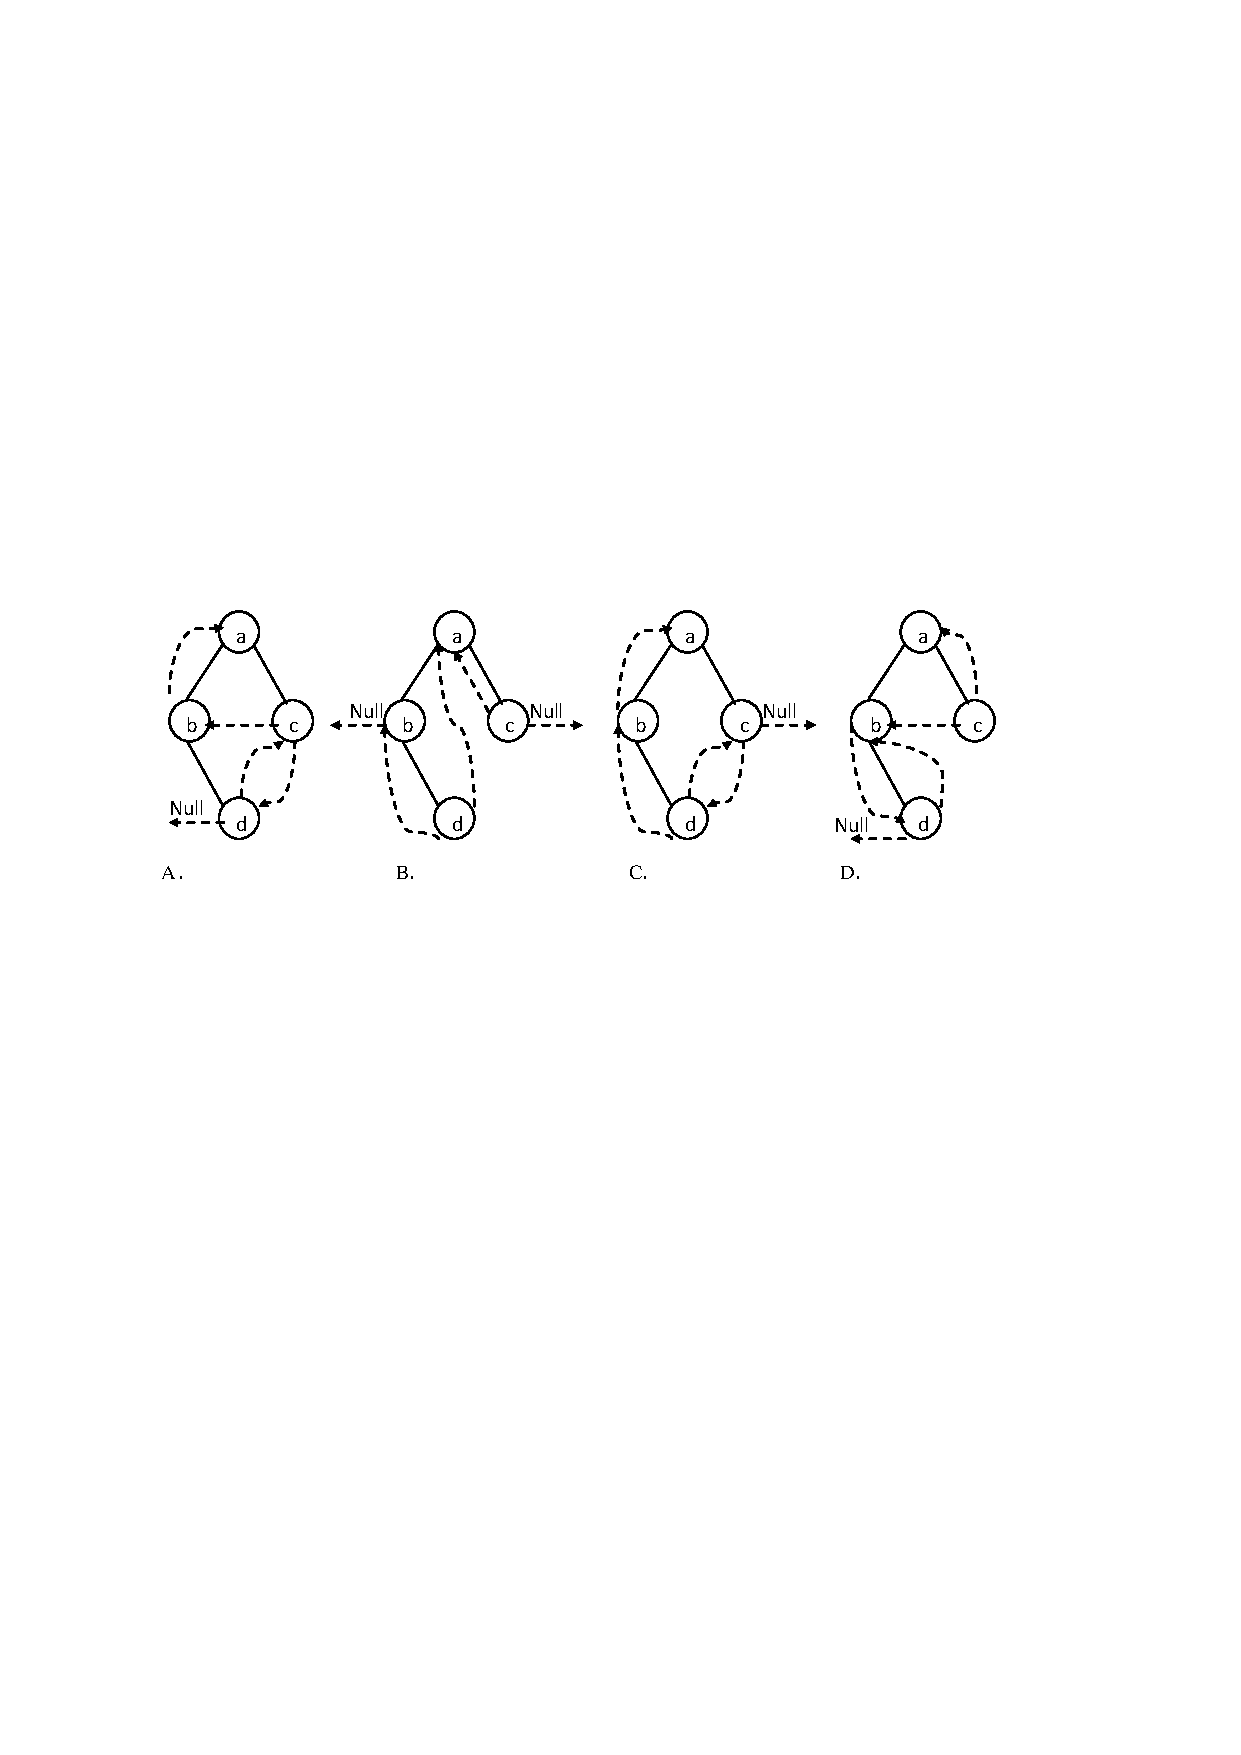
\includegraphics[width=.65\linewidth,height=.4\textheight,keepaspectratio]{../assets/figures/2010-complete-p001-b005.pdf}\end{center}

4. 在右图所示的平衡二叉树中，插入关键字 48 后得到一棵新平衡二叉树。在新平衡二叉树中，关键字 37 所在结点的左、右子结点中保存的关键字分别是\_\_\_\_\_\_。


\begin{center}\begin{tabular}{>{\raggedright\arraybackslash}p{\dimexpr(\linewidth-8\tabcolsep)/4\relax}>{\raggedright\arraybackslash}p{\dimexpr(\linewidth-8\tabcolsep)/4\relax}>{\raggedright\arraybackslash}p{\dimexpr(\linewidth-8\tabcolsep)/4\relax}>{\raggedright\arraybackslash}p{\dimexpr(\linewidth-8\tabcolsep)/4\relax}}
\textbf{A.} 13，48 & \textbf{B.} 24，48 & \textbf{C.} 24，53 & \textbf{D.} 24，90\\[.35em]\end{tabular}\end{center}

\begin{center}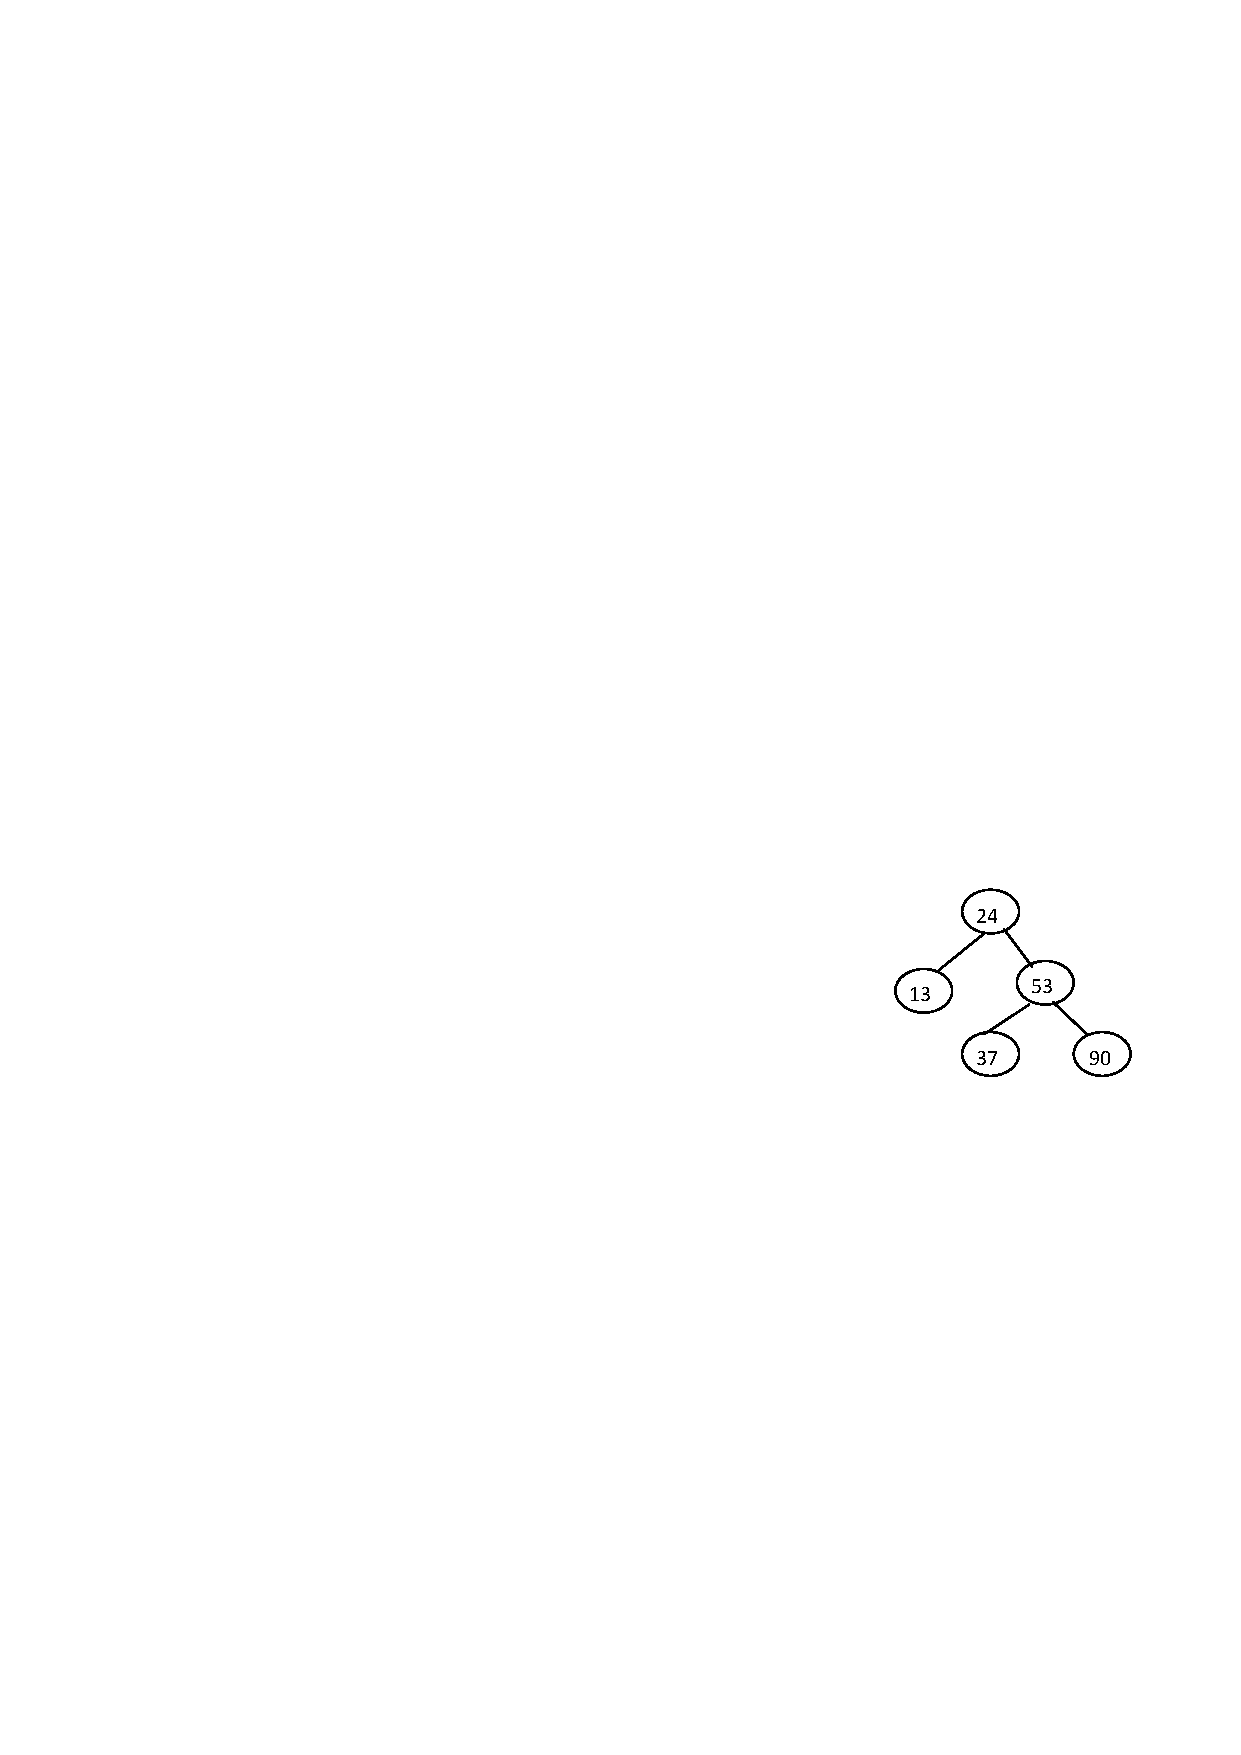
\includegraphics[width=.65\linewidth,height=.4\textheight,keepaspectratio]{../assets/figures/2010-complete-p001-b007.pdf}\end{center}

5. 在一棵度为 4 的树 T 中，若有 20 个度为 4 的结点，10 个度为 3 的结点，1 个度为 2 的结点，10 个度为 1 的结点，则树 T 的叶结点个数是\_\_\_\_\_\_。


\begin{center}\begin{tabular}{>{\raggedright\arraybackslash}p{\dimexpr(\linewidth-8\tabcolsep)/4\relax}>{\raggedright\arraybackslash}p{\dimexpr(\linewidth-8\tabcolsep)/4\relax}>{\raggedright\arraybackslash}p{\dimexpr(\linewidth-8\tabcolsep)/4\relax}>{\raggedright\arraybackslash}p{\dimexpr(\linewidth-8\tabcolsep)/4\relax}}
\textbf{A.} 41 & \textbf{B.} 82 & \textbf{C.} 113 & \textbf{D.} 122\\[.35em]\end{tabular}\end{center}

6. 对n（n≥2）个权值均不相同的字符构造成哈夫曼树。下列关于该哈夫曼树的叙述中，错误．．的是\_\_\_\_\_\_。


\begin{center}\begin{tabular}{>{\raggedright\arraybackslash}p{\dimexpr(\linewidth-4\tabcolsep)/2\relax}>{\raggedright\arraybackslash}p{\dimexpr(\linewidth-4\tabcolsep)/2\relax}}
\textbf{A.} 该树一定是一棵完全二叉树。 & \textbf{B.} 树中一定没有度为1 的结点。\\[.35em]
\textbf{C.} 树中两个权值最小的结点一定是兄弟结点。 & \textbf{D.} 树中任一非叶结点的权值一定不小于下一层任一结点的权值。\\[.35em]\end{tabular}\end{center}

7. 若无向图 \(\displaystyle G=(V,\allowbreak E)\) 中含有 7 个顶点，要保证图 G 在任何情况下都是连通的，则需要的边数最少是\_\_\_\_\_\_。


\begin{center}\begin{tabular}{>{\raggedright\arraybackslash}p{\dimexpr(\linewidth-8\tabcolsep)/4\relax}>{\raggedright\arraybackslash}p{\dimexpr(\linewidth-8\tabcolsep)/4\relax}>{\raggedright\arraybackslash}p{\dimexpr(\linewidth-8\tabcolsep)/4\relax}>{\raggedright\arraybackslash}p{\dimexpr(\linewidth-8\tabcolsep)/4\relax}}
\textbf{A.} 6 & \textbf{B.} 15 & \textbf{C.} 16 & \textbf{D.} 21\\[.35em]\end{tabular}\end{center}

8. 对右图进行拓扑排序，可以得到不同的拓扑序列的个数是\_\_\_\_\_\_。


\begin{center}\begin{tabular}{>{\raggedright\arraybackslash}p{\dimexpr(\linewidth-8\tabcolsep)/4\relax}>{\raggedright\arraybackslash}p{\dimexpr(\linewidth-8\tabcolsep)/4\relax}>{\raggedright\arraybackslash}p{\dimexpr(\linewidth-8\tabcolsep)/4\relax}>{\raggedright\arraybackslash}p{\dimexpr(\linewidth-8\tabcolsep)/4\relax}}
\textbf{A.} 4 & \textbf{B.} 3 & \textbf{C.} 2 & \textbf{D.} 1\\[.35em]\end{tabular}\end{center}

\begin{center}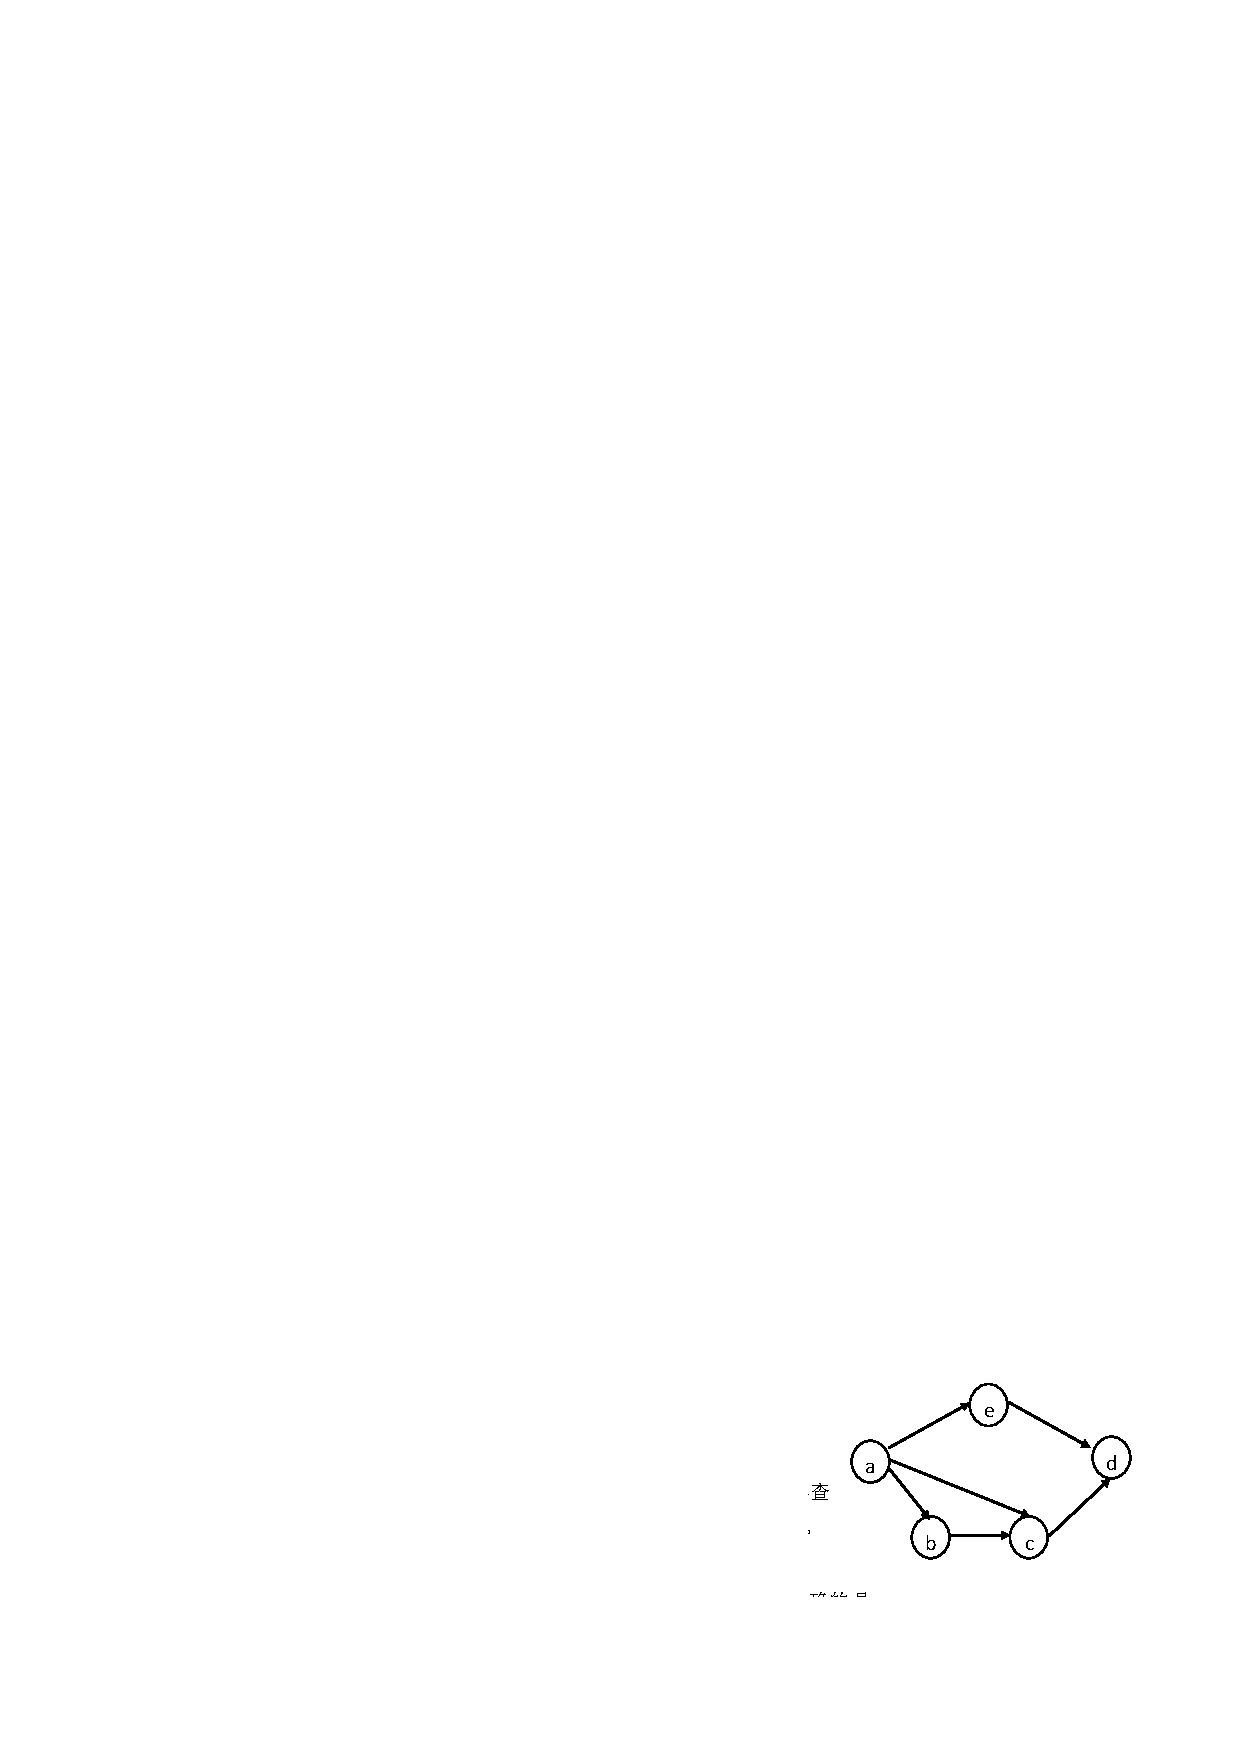
\includegraphics[width=.65\linewidth,height=.4\textheight,keepaspectratio]{../assets/figures/2010-complete-p001-b012.pdf}\end{center}

9. 已知一个长度为16 的顺序表L，其元素按关键字有序排列。若采用折半查找法查找一个L 中不存在的元素，则关键字的比较次数最多的是\_\_\_\_\_。


\begin{center}\begin{tabular}{>{\raggedright\arraybackslash}p{\dimexpr(\linewidth-8\tabcolsep)/4\relax}>{\raggedright\arraybackslash}p{\dimexpr(\linewidth-8\tabcolsep)/4\relax}>{\raggedright\arraybackslash}p{\dimexpr(\linewidth-8\tabcolsep)/4\relax}>{\raggedright\arraybackslash}p{\dimexpr(\linewidth-8\tabcolsep)/4\relax}}
\textbf{A.} 4 & \textbf{B.} 5 & \textbf{C.} 6 & \textbf{D.} 7\\[.35em]\end{tabular}\end{center}

10. 采用递归方式对顺序表进行快速排序。下列关于递归次数的叙述中，正确的是\_\_\_\_\_\_。


\begin{center}\begin{tabular}{>{\raggedright\arraybackslash}p{\dimexpr(\linewidth-4\tabcolsep)/2\relax}>{\raggedright\arraybackslash}p{\dimexpr(\linewidth-4\tabcolsep)/2\relax}}
\textbf{A.} 递归次数与初始数据的排列次序无关。 & \\[.35em]\end{tabular}\end{center}

\begin{center}\begin{tabular}{>{\raggedright\arraybackslash}p{\dimexpr(\linewidth-4\tabcolsep)/2\relax}>{\raggedright\arraybackslash}p{\dimexpr(\linewidth-4\tabcolsep)/2\relax}}
\textbf{B.} 每次划分后，先处理较长的分区可以减少递归次数。 & \textbf{C.} 每次划分后，先处理较短的分区可以减少递归次数。\\[.35em]
\textbf{D.} 递归次数与每次划分后得到的分区的处理顺序无关。 & \\[.35em]\end{tabular}\end{center}

11. 对一组数据(2，12，16，88，5，10)进行排序，若前三趟排序结果如下：第一趟排序结果：2，12，16，5，10，88第二趟排序结果：2，12，5，10，16，88第三趟排序结果：2，5，10，12，16，88则采用的排序方法可能是\_\_\_\_\_\_。


\begin{center}\begin{tabular}{>{\raggedright\arraybackslash}p{\dimexpr(\linewidth-8\tabcolsep)/4\relax}>{\raggedright\arraybackslash}p{\dimexpr(\linewidth-8\tabcolsep)/4\relax}>{\raggedright\arraybackslash}p{\dimexpr(\linewidth-8\tabcolsep)/4\relax}>{\raggedright\arraybackslash}p{\dimexpr(\linewidth-8\tabcolsep)/4\relax}}
\textbf{A.} 起泡排序 & \textbf{B.} 希尔排序 & \textbf{C.} 归并排序 & \textbf{D.} 基数排序\\[.35em]\end{tabular}\end{center}

12. 下列选项中，能缩短程序执行时间的措施是 。Ⅰ. 提高CPU 时钟频率 Ⅱ. 优化数据通路结构Ⅲ. 对程序进行编译优化


\begin{center}\begin{tabular}{>{\raggedright\arraybackslash}p{\dimexpr(\linewidth-8\tabcolsep)/4\relax}>{\raggedright\arraybackslash}p{\dimexpr(\linewidth-8\tabcolsep)/4\relax}>{\raggedright\arraybackslash}p{\dimexpr(\linewidth-8\tabcolsep)/4\relax}>{\raggedright\arraybackslash}p{\dimexpr(\linewidth-8\tabcolsep)/4\relax}}
\textbf{A.} 仅Ⅰ和Ⅱ & \textbf{B.} 仅Ⅰ和Ⅲ & \textbf{C.} 仅Ⅱ和Ⅲ & \textbf{D.} Ⅰ、Ⅱ和Ⅲ\\[.35em]\end{tabular}\end{center}

13. 假定有4 个整数用8 位补码分别表示r1=FEH，r2=F2H，r3=90H，r4=F8H，若将运算结果存放在一个8 位寄存器中，则下列运算中会发生溢出的是 。


\begin{center}\begin{tabular}{>{\raggedright\arraybackslash}p{\dimexpr(\linewidth-8\tabcolsep)/4\relax}>{\raggedright\arraybackslash}p{\dimexpr(\linewidth-8\tabcolsep)/4\relax}>{\raggedright\arraybackslash}p{\dimexpr(\linewidth-8\tabcolsep)/4\relax}>{\raggedright\arraybackslash}p{\dimexpr(\linewidth-8\tabcolsep)/4\relax}}
\textbf{A.} r1 x r2 & \textbf{B.} r2 x r3 & \textbf{C.} r1 x r4 & \textbf{D.} r2 x r4\\[.35em]\end{tabular}\end{center}

14. 假定变量 i、f 和 d 的数据类型分别为 int、float 和 double（int 用补码表示，float 和 double 分别用 IEEE754 单精度和双精度浮点数格式表示），已知 \(\displaystyle i=785,\allowbreak f=1.5678\times10^3,\allowbreak d=1.5\times10^{100}\)。若在 32 位机器中执行下列关系表达式，则结果为“真”的是\_\_\_\_\_\_。（I）i == (int)(float)i （II）f == (float)(int)f （III）f == (float)(double)f （IV）(d+f)-d == f


\begin{center}\begin{tabular}{>{\raggedright\arraybackslash}p{\dimexpr(\linewidth-8\tabcolsep)/4\relax}>{\raggedright\arraybackslash}p{\dimexpr(\linewidth-8\tabcolsep)/4\relax}>{\raggedright\arraybackslash}p{\dimexpr(\linewidth-8\tabcolsep)/4\relax}>{\raggedright\arraybackslash}p{\dimexpr(\linewidth-8\tabcolsep)/4\relax}}
\textbf{A.} 仅 I 和 II & \textbf{B.} 仅 I 和 III & \textbf{C.} 仅 II 和 III & \textbf{D.} 仅 III 和 IV\\[.35em]\end{tabular}\end{center}

15. 15. 假定用若干个 \(\displaystyle 2\mathrm{K}\times4\) 位的芯片组成一个 \(\displaystyle 8\mathrm{K}\times8\) 位的存储器，则地址 0B1FH 所在芯片的最小地址是\_\_\_\_\_\_。


\begin{center}\begin{tabular}{>{\raggedright\arraybackslash}p{\dimexpr(\linewidth-8\tabcolsep)/4\relax}>{\raggedright\arraybackslash}p{\dimexpr(\linewidth-8\tabcolsep)/4\relax}>{\raggedright\arraybackslash}p{\dimexpr(\linewidth-8\tabcolsep)/4\relax}>{\raggedright\arraybackslash}p{\dimexpr(\linewidth-8\tabcolsep)/4\relax}}
\textbf{A.} 0000H & \textbf{B.} 0600H & \textbf{C.} 0700H & \textbf{D.} 0800H\\[.35em]\end{tabular}\end{center}

16. 下列有关RAM 和ROM 的叙述中，正确的是 。I RAM 是易失性存储器，ROM 是非易失性存储器II RAM 和ROM 都采用随机存取方式进行信息访问III RAM 和ROM 都可用作CacheIV RAM 和ROM 都需要进行刷新


\begin{center}\begin{tabular}{>{\raggedright\arraybackslash}p{\dimexpr(\linewidth-8\tabcolsep)/4\relax}>{\raggedright\arraybackslash}p{\dimexpr(\linewidth-8\tabcolsep)/4\relax}>{\raggedright\arraybackslash}p{\dimexpr(\linewidth-8\tabcolsep)/4\relax}>{\raggedright\arraybackslash}p{\dimexpr(\linewidth-8\tabcolsep)/4\relax}}
\textbf{A.} 仅I 和II & \textbf{B.} 仅II 和III & \textbf{C.} 仅I,II 和IV & \textbf{D.} 仅II，III 和IV\\[.35em]\end{tabular}\end{center}

17. 下列命中组合情况中，一次访存过程中不．可能发生的是 。


\begin{center}\begin{tabular}{>{\raggedright\arraybackslash}p{\dimexpr(\linewidth-4\tabcolsep)/2\relax}>{\raggedright\arraybackslash}p{\dimexpr(\linewidth-4\tabcolsep)/2\relax}}
\textbf{A.} TLB 未命中，Cache 未命中，Page 未命中 & \textbf{B.} TLB 未命中，Cache 命中，Page 命中\\[.35em]
\textbf{C.} TLB 命中，Cache 未命中，Page 命中 & \textbf{D.} TLB 命中，Cache 命中，Page 未命中\\[.35em]\end{tabular}\end{center}

18. 下列寄存器中，汇编语言程序员可见的是 。


\begin{center}\begin{tabular}{>{\raggedright\arraybackslash}p{\dimexpr(\linewidth-4\tabcolsep)/2\relax}>{\raggedright\arraybackslash}p{\dimexpr(\linewidth-4\tabcolsep)/2\relax}}
\textbf{A.} 存储器地址寄存器(MAR) & \textbf{B.} 程序计数器(PC)\\[.35em]
\textbf{C.} 存储器数据寄存器(MDR) & \textbf{D.} 指令寄存器(IR)\\[.35em]\end{tabular}\end{center}

19. 下列选项中，不．会引起指令流水线阻塞的是 。


\begin{center}\begin{tabular}{>{\raggedright\arraybackslash}p{\dimexpr(\linewidth-8\tabcolsep)/4\relax}>{\raggedright\arraybackslash}p{\dimexpr(\linewidth-8\tabcolsep)/4\relax}>{\raggedright\arraybackslash}p{\dimexpr(\linewidth-8\tabcolsep)/4\relax}>{\raggedright\arraybackslash}p{\dimexpr(\linewidth-8\tabcolsep)/4\relax}}
\textbf{A.} 数据旁路（转发） & \textbf{B.} 数据相关 & \textbf{C.} 条件转移 & \textbf{D.} 资源冲突\\[.35em]\end{tabular}\end{center}

20. 下列选项中的英文缩写均为总线标准的是\_\_\_\_\_\_。


\begin{center}\begin{tabular}{>{\raggedright\arraybackslash}p{\dimexpr(\linewidth-4\tabcolsep)/2\relax}>{\raggedright\arraybackslash}p{\dimexpr(\linewidth-4\tabcolsep)/2\relax}}
\textbf{A.} PCI、CRT、USB、EISA & \textbf{B.} ISA、CPI、VESA、EISA\\[.35em]
\textbf{C.} ISA、SCSI、RAM、MIPS & \textbf{D.} ISA、EISA、PCI、PCI-Express\\[.35em]\end{tabular}\end{center}

21. 单级中断系统中，中断服务程序内的执行顺序是\_\_\_\_\_\_。I 保护现场 II 开中断 III 关中断 IV 保存断点V 中断事件处理 VI 恢复现场 VII 中断返回


\begin{center}\begin{tabular}{>{\raggedright\arraybackslash}p{\dimexpr(\linewidth-4\tabcolsep)/2\relax}>{\raggedright\arraybackslash}p{\dimexpr(\linewidth-4\tabcolsep)/2\relax}}
\textbf{A.} I->V->VI->II->VII & \textbf{B.} III->I->V->VII\\[.35em]
\textbf{C.} III->IV->V->VI->VII & \textbf{D.} IV->I->V->VI->VII\\[.35em]\end{tabular}\end{center}

22. 假定一台计算机的显示存储器用DRAM 芯片实现，若要求显示分辨率为1600*1200，颜色深度为24 位，帧频为85HZ，显存总带宽的50\%用来刷新屏幕，则需要的显存总带宽至少约为\_\_\_\_\_\_。


\begin{center}\begin{tabular}{>{\raggedright\arraybackslash}p{\dimexpr(\linewidth-8\tabcolsep)/4\relax}>{\raggedright\arraybackslash}p{\dimexpr(\linewidth-8\tabcolsep)/4\relax}>{\raggedright\arraybackslash}p{\dimexpr(\linewidth-8\tabcolsep)/4\relax}>{\raggedright\arraybackslash}p{\dimexpr(\linewidth-8\tabcolsep)/4\relax}}
\textbf{A.} 245Mbps & \textbf{B.} 979Mbps & \textbf{C.} 1 958Mbps & \textbf{D.} 7 834Mbps\\[.35em]\end{tabular}\end{center}

23. 下列选项中，操作系统提供给应用程序的接口是\_\_\_\_\_。


\begin{center}\begin{tabular}{>{\raggedright\arraybackslash}p{\dimexpr(\linewidth-8\tabcolsep)/4\relax}>{\raggedright\arraybackslash}p{\dimexpr(\linewidth-8\tabcolsep)/4\relax}>{\raggedright\arraybackslash}p{\dimexpr(\linewidth-8\tabcolsep)/4\relax}>{\raggedright\arraybackslash}p{\dimexpr(\linewidth-8\tabcolsep)/4\relax}}
\textbf{A.} 系统调用 & \textbf{B.} 中断 & \textbf{C.} 库函数 & \textbf{D.} 原语\\[.35em]\end{tabular}\end{center}

24. 下列选项中，导致创建新进程的操作是\_\_\_\_\_\_。Ⅰ用户登录成功 Ⅱ设备分配 Ⅲ启动程序执行


\begin{center}\begin{tabular}{>{\raggedright\arraybackslash}p{\dimexpr(\linewidth-8\tabcolsep)/4\relax}>{\raggedright\arraybackslash}p{\dimexpr(\linewidth-8\tabcolsep)/4\relax}>{\raggedright\arraybackslash}p{\dimexpr(\linewidth-8\tabcolsep)/4\relax}>{\raggedright\arraybackslash}p{\dimexpr(\linewidth-8\tabcolsep)/4\relax}}
\textbf{A.} 仅Ⅰ和Ⅱ & \textbf{B.} 仅Ⅱ和Ⅲ & \textbf{C.} 仅Ⅰ和Ⅲ & \textbf{D.} Ⅰ、Ⅱ和Ⅲ\\[.35em]\end{tabular}\end{center}

25. 设与某资源关联的信号量初值为3，当前值为1。若M 表示该资源的可用个数，N 表示等待该资源的进程数，则M、N 分别是\_\_\_\_\_\_。


\begin{center}\begin{tabular}{>{\raggedright\arraybackslash}p{\dimexpr(\linewidth-8\tabcolsep)/4\relax}>{\raggedright\arraybackslash}p{\dimexpr(\linewidth-8\tabcolsep)/4\relax}>{\raggedright\arraybackslash}p{\dimexpr(\linewidth-8\tabcolsep)/4\relax}>{\raggedright\arraybackslash}p{\dimexpr(\linewidth-8\tabcolsep)/4\relax}}
\textbf{A.} 0、1 & \textbf{B.} 1、0 & \textbf{C.} 1、2 & \textbf{D.} 2、0\\[.35em]\end{tabular}\end{center}

26. 下列选项中，降低进程优先级的合理时机是\_\_\_\_\_。


\begin{center}\begin{tabular}{>{\raggedright\arraybackslash}p{\dimexpr(\linewidth-4\tabcolsep)/2\relax}>{\raggedright\arraybackslash}p{\dimexpr(\linewidth-4\tabcolsep)/2\relax}}
\textbf{A.} 进程的时间片用完 & \textbf{B.} 进程刚完成I/O，进入就绪列队\\[.35em]
\textbf{C.} 进程长期处于就绪列队中 & \textbf{D.} 进程从就绪态转为运行态\\[.35em]\end{tabular}\end{center}

27. 进程 P0 和 P1 的共享变量定义及其初值为：


\begin{Verbatim}[breaklines,breakanywhere,fontsize=\small]
boolean flag[2];
int turn = 0;
flag[0] = FALSE; flag[1] = FALSE;
\end{Verbatim}

若进程 P0 和 P1 访问临界资源的类 C 伪代码实现如下：


\begin{Verbatim}[breaklines,breakanywhere,fontsize=\small]
void P0()    // 进程 P0
{
    while (TRUE) {
        flag[0] = TRUE; turn = 1;
        while (flag[1] && (turn == 1))
            ;
        临界区;
        flag[0] = FALSE;
    }
}
\end{Verbatim}

\begin{Verbatim}[breaklines,breakanywhere,fontsize=\small]
void P1()    // 进程 P1
{
    while (TRUE) {
        flag[1] = TRUE; turn = 0;
        while (flag[0] && (turn == 0))
            ;
        临界区;
        flag[1] = FALSE;
    }
}
\end{Verbatim}

则并发执行进程P0 和P1 时产生的情形是\_\_\_\_\_\_。


\begin{center}\begin{tabular}{>{\raggedright\arraybackslash}p{\dimexpr(\linewidth-4\tabcolsep)/2\relax}>{\raggedright\arraybackslash}p{\dimexpr(\linewidth-4\tabcolsep)/2\relax}}
\textbf{A.} 不能保证进程互斥进入临界区，会出现“饥饿”现象 & \textbf{B.} 不能保证进程互斥进入临界区，不会出现“饥饿”现象\\[.35em]
\textbf{C.} 能保证进程互斥进入临界区，会出现“饥饿”现象 & \textbf{D.} 能保证进程互斥进入临界区，不会出现“饥饿”现象\\[.35em]\end{tabular}\end{center}

28. 某基于动态分区存储管理的计算机，其主存容量为55MB(初始为空闲)，采用最佳适配(Best Fit)算法，分配和释放的顺序为：分配15MB，分配30MB，释放15MB，分配8MB，分配6MB，此时主存中最大空闲分区的大小是\_\_\_\_\_\_。


\begin{center}\begin{tabular}{>{\raggedright\arraybackslash}p{\dimexpr(\linewidth-8\tabcolsep)/4\relax}>{\raggedright\arraybackslash}p{\dimexpr(\linewidth-8\tabcolsep)/4\relax}>{\raggedright\arraybackslash}p{\dimexpr(\linewidth-8\tabcolsep)/4\relax}>{\raggedright\arraybackslash}p{\dimexpr(\linewidth-8\tabcolsep)/4\relax}}
\textbf{A.} 7MB & \textbf{B.} 9MB & \textbf{C.} 10MB & \textbf{D.} 15MB\\[.35em]\end{tabular}\end{center}

29. 某计算机采用二级页表的分页存储管理方式，按字节编址，页大小为 \(\displaystyle 2^{10}\) 字节，页表项大小为 2 字节，逻辑地址结构为：


\begin{center}\begin{adjustbox}{max width=\linewidth}\begin{tabular}{|>{\raggedright\arraybackslash}p{\dimexpr(\linewidth-6\tabcolsep-4\arrayrulewidth)/3\relax}|>{\raggedright\arraybackslash}p{\dimexpr(\linewidth-6\tabcolsep-4\arrayrulewidth)/3\relax}|>{\raggedright\arraybackslash}p{\dimexpr(\linewidth-6\tabcolsep-4\arrayrulewidth)/3\relax}|}\hline
页目录号 & 页号 & 页内偏移量\\\hline\end{tabular}\end{adjustbox}\end{center}

逻辑地址空间大小为 \(\displaystyle 2^{16}\) 页，则表示整个逻辑地址空间的页目录表中包含表项的个数至少是\_\_\_\_\_\_。


\begin{center}\begin{tabular}{>{\raggedright\arraybackslash}p{\dimexpr(\linewidth-8\tabcolsep)/4\relax}>{\raggedright\arraybackslash}p{\dimexpr(\linewidth-8\tabcolsep)/4\relax}>{\raggedright\arraybackslash}p{\dimexpr(\linewidth-8\tabcolsep)/4\relax}>{\raggedright\arraybackslash}p{\dimexpr(\linewidth-8\tabcolsep)/4\relax}}
\textbf{A.} 64 & \textbf{B.} 128 & \textbf{C.} 256 & \textbf{D.} 512\\[.35em]\end{tabular}\end{center}

30. 设文件索引节点中有7 个地址项，其中4 个地址项是直接地址索引，2 个地址项是一级间接地址索引，1个地址项是二级间接地址索引，每个地址项大小为4 字节。若磁盘索引块和磁盘数据块大小均为256 字节，则可表示的单个文件最大长度是\_\_\_\_\_\_。


\begin{center}\begin{tabular}{>{\raggedright\arraybackslash}p{\dimexpr(\linewidth-8\tabcolsep)/4\relax}>{\raggedright\arraybackslash}p{\dimexpr(\linewidth-8\tabcolsep)/4\relax}>{\raggedright\arraybackslash}p{\dimexpr(\linewidth-8\tabcolsep)/4\relax}>{\raggedright\arraybackslash}p{\dimexpr(\linewidth-8\tabcolsep)/4\relax}}
\textbf{A.} 33 KB & \textbf{B.} 519 KB & \textbf{C.} 1 057 KB & \textbf{D.} 16 513 KB\\[.35em]\end{tabular}\end{center}

31. 设置当前工作目录的主要目的是\_\_\_\_\_\_\_。


\begin{center}\begin{tabular}{>{\raggedright\arraybackslash}p{\dimexpr(\linewidth-4\tabcolsep)/2\relax}>{\raggedright\arraybackslash}p{\dimexpr(\linewidth-4\tabcolsep)/2\relax}}
\textbf{A.} 节省外存空间 & \textbf{B.} 节省内存空间\\[.35em]
\textbf{C.} 加快文件的检索速度 & \textbf{D.} 加快文件的读/写速度\\[.35em]\end{tabular}\end{center}

32. 本地用户通过键盘登陆系统时，首先获得键盘输入信息的程序是\_\_\_\_\_\_。


\begin{center}\begin{tabular}{>{\raggedright\arraybackslash}p{\dimexpr(\linewidth-8\tabcolsep)/4\relax}>{\raggedright\arraybackslash}p{\dimexpr(\linewidth-8\tabcolsep)/4\relax}>{\raggedright\arraybackslash}p{\dimexpr(\linewidth-8\tabcolsep)/4\relax}>{\raggedright\arraybackslash}p{\dimexpr(\linewidth-8\tabcolsep)/4\relax}}
\textbf{A.} 命令解释程序 & \textbf{B.} 中断处理程序 & \textbf{C.} 系统调用服务程序 & \textbf{D.} 用户登录程序\\[.35em]\end{tabular}\end{center}

33. 下列选项中，不．属于网络体系结构所描述的内容是\_\_\_\_\_\_。


\begin{center}\begin{tabular}{>{\raggedright\arraybackslash}p{\dimexpr(\linewidth-4\tabcolsep)/2\relax}>{\raggedright\arraybackslash}p{\dimexpr(\linewidth-4\tabcolsep)/2\relax}}
\textbf{A.} 网络的层次 & \textbf{B.} 每一层使用的协议\\[.35em]
\textbf{C.} 协议的内部实现细节 & \textbf{D.} 每一层必须完成的功能\\[.35em]\end{tabular}\end{center}

34. 在下图所示的采用“存储-转发”方式的分组交换网络中，所有链路的数据传输速率为100Mbps，分组大小为1000B，其中分组头大小为20B。若主机H1 向主机H2 发送一个大小为980 000B 的文件，则在不考虑分组拆装时间和传播延迟的情况下，从H1 发送开始到H2 接收完为止，需要的时间至少．．是\_\_\_\_\_\_。


\begin{center}\begin{tabular}{>{\raggedright\arraybackslash}p{\dimexpr(\linewidth-8\tabcolsep)/4\relax}>{\raggedright\arraybackslash}p{\dimexpr(\linewidth-8\tabcolsep)/4\relax}>{\raggedright\arraybackslash}p{\dimexpr(\linewidth-8\tabcolsep)/4\relax}>{\raggedright\arraybackslash}p{\dimexpr(\linewidth-8\tabcolsep)/4\relax}}
\textbf{A.} 80 ms & \textbf{B.} 80.\allowbreak{}08 ms & \textbf{C.} 80.\allowbreak{}16 ms & \textbf{D.} 80.\allowbreak{}24 ms\\[.35em]\end{tabular}\end{center}

\begin{center}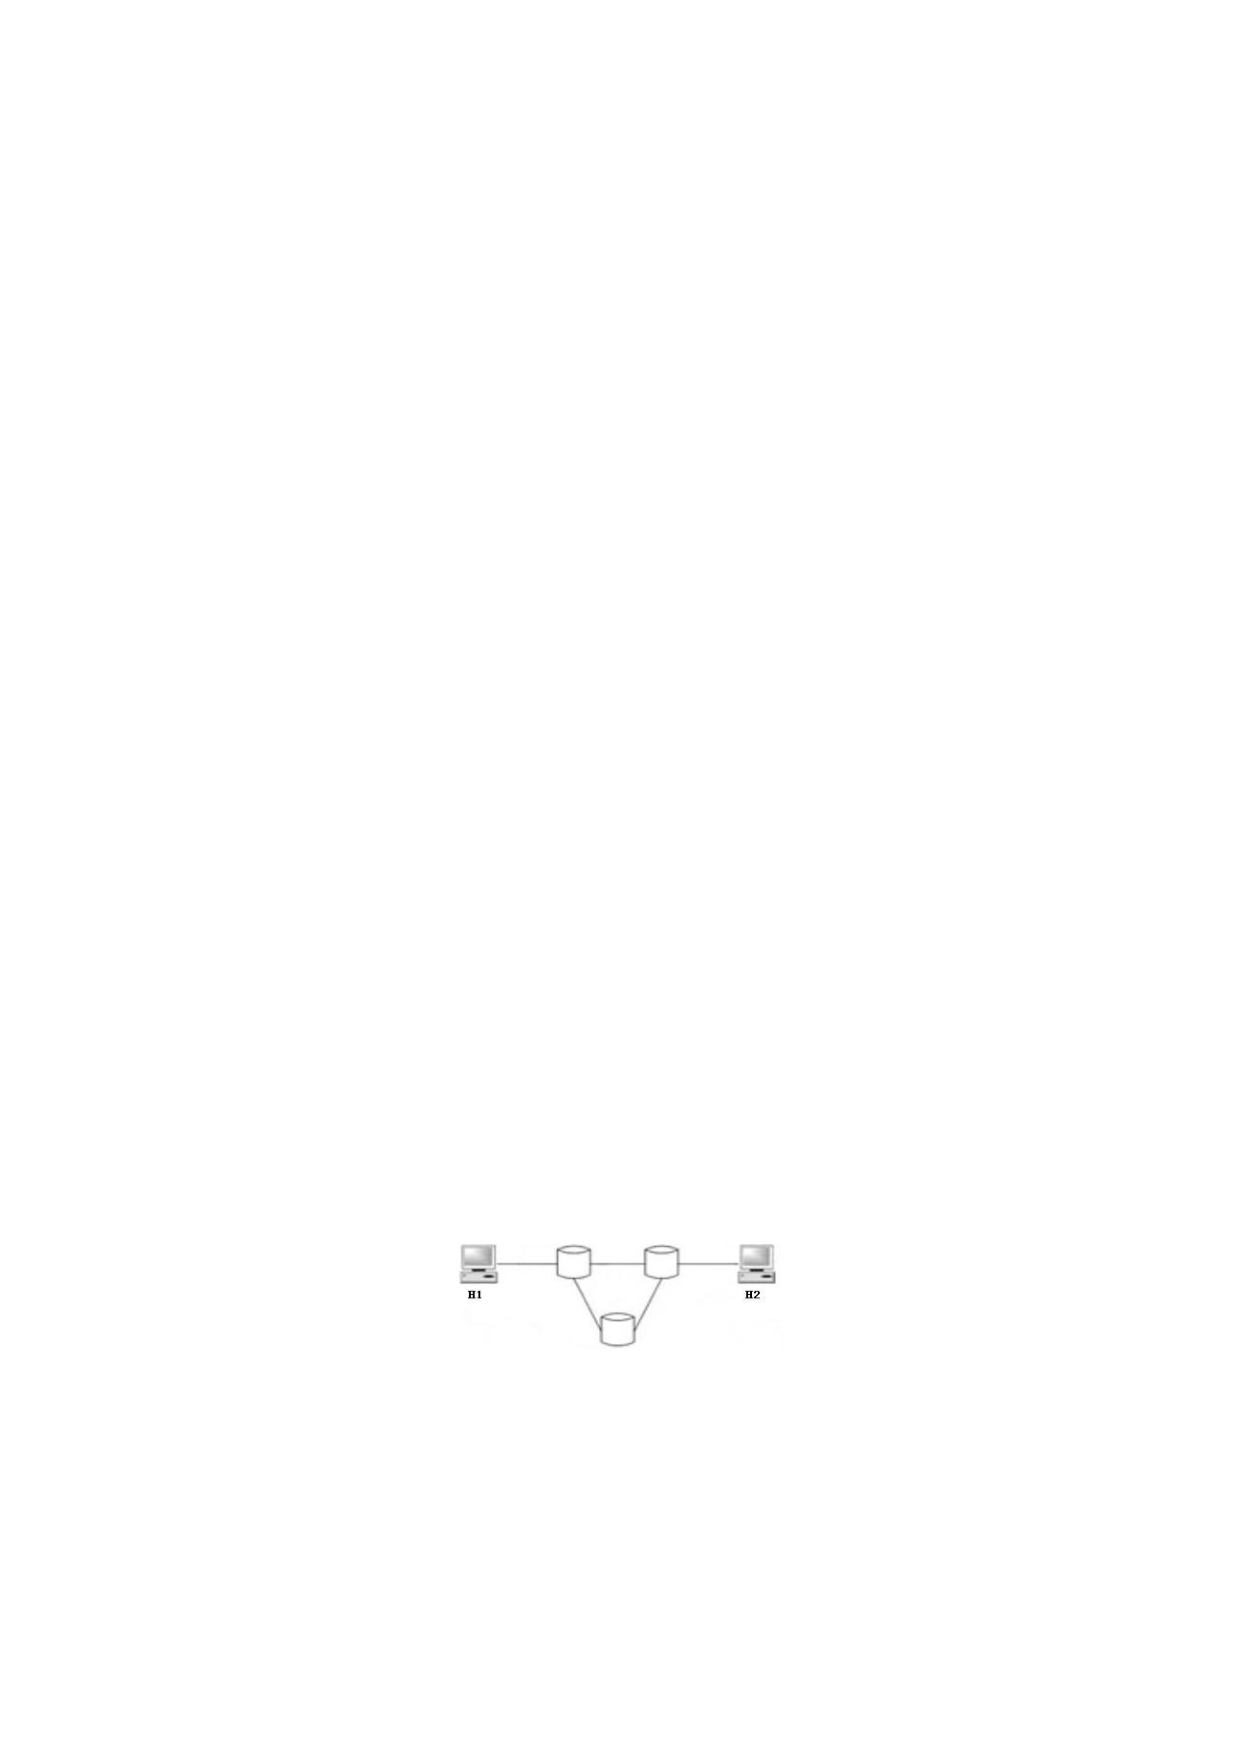
\includegraphics[width=.65\linewidth,height=.4\textheight,keepaspectratio]{../assets/figures/2010-complete-p004-b010.pdf}\end{center}

35. 某自治系统内采用RIP 协议，若该自治系统内的路由器R1 收到其邻居路由器R2 的距离矢量，距离矢量中包含信息<net1, 16>，则能得出的结论是\_\_\_\_\_\_。


\begin{center}\begin{tabular}{>{\raggedright\arraybackslash}p{\dimexpr(\linewidth-4\tabcolsep)/2\relax}>{\raggedright\arraybackslash}p{\dimexpr(\linewidth-4\tabcolsep)/2\relax}}
\textbf{A.} R2 可以经过R1 到达net1，跳数为17 & \textbf{B.} R2 可以到达net1，跳数为16\\[.35em]
\textbf{C.} R1 可以经过R2 到达net1，跳数为17 & \textbf{D.} R1 不能经过R2 到达net1\\[.35em]\end{tabular}\end{center}

36. 若路由器R 因为拥塞丢弃IP 分组，则此时R 可向发出该IP 分组的源主机发送的ICMP 报文类型是\_\_\_\_\_\_。


\begin{center}\begin{tabular}{>{\raggedright\arraybackslash}p{\dimexpr(\linewidth-8\tabcolsep)/4\relax}>{\raggedright\arraybackslash}p{\dimexpr(\linewidth-8\tabcolsep)/4\relax}>{\raggedright\arraybackslash}p{\dimexpr(\linewidth-8\tabcolsep)/4\relax}>{\raggedright\arraybackslash}p{\dimexpr(\linewidth-8\tabcolsep)/4\relax}}
\textbf{A.} 路由重定向 & \textbf{B.} 目的不可达 & \textbf{C.} 源点抑制 & \textbf{D.} 超时\\[.35em]\end{tabular}\end{center}

37. 某网络的IP 地址空间为192.168.5.0/24，采用定长子网划分，子网掩码为255.255.255.248，则该网络中的最大子网个数、每个子网内的最大可分配地址个数分别是\_\_\_\_\_\_。


\begin{center}\begin{tabular}{>{\raggedright\arraybackslash}p{\dimexpr(\linewidth-8\tabcolsep)/4\relax}>{\raggedright\arraybackslash}p{\dimexpr(\linewidth-8\tabcolsep)/4\relax}>{\raggedright\arraybackslash}p{\dimexpr(\linewidth-8\tabcolsep)/4\relax}>{\raggedright\arraybackslash}p{\dimexpr(\linewidth-8\tabcolsep)/4\relax}}
\textbf{A.} 32，8 & \textbf{B.} 32，6 & \textbf{C.} 8，32 & \textbf{D.} 8，30\\[.35em]\end{tabular}\end{center}

38. 下列网络设备中，能够抑制广播风暴的是\_\_\_\_\_\_。Ⅰ中继器 Ⅱ集线器 Ⅲ网桥 Ⅳ路由器


\begin{center}\begin{tabular}{>{\raggedright\arraybackslash}p{\dimexpr(\linewidth-8\tabcolsep)/4\relax}>{\raggedright\arraybackslash}p{\dimexpr(\linewidth-8\tabcolsep)/4\relax}>{\raggedright\arraybackslash}p{\dimexpr(\linewidth-8\tabcolsep)/4\relax}>{\raggedright\arraybackslash}p{\dimexpr(\linewidth-8\tabcolsep)/4\relax}}
\textbf{A.} 仅Ⅰ和Ⅱ & \textbf{B.} 仅Ⅲ & \textbf{C.} 仅Ⅲ和Ⅳ & \textbf{D.} 仅Ⅳ\\[.35em]\end{tabular}\end{center}

39. 主机甲和主机乙之间已建立了一个TCP 连接，TCP 最大段长度为1 000 字节。若主机甲的当前拥塞窗口为4 000 字节，在主机甲向主机乙连续发送两个最大段后，成功收到主机乙发送的第一个段的确认段，确认段中通告的接收窗口大小为2 000 字节，则此时主机甲还可以向主机乙发送的最大字节数是\_\_\_\_\_\_。


\begin{center}\begin{tabular}{>{\raggedright\arraybackslash}p{\dimexpr(\linewidth-8\tabcolsep)/4\relax}>{\raggedright\arraybackslash}p{\dimexpr(\linewidth-8\tabcolsep)/4\relax}>{\raggedright\arraybackslash}p{\dimexpr(\linewidth-8\tabcolsep)/4\relax}>{\raggedright\arraybackslash}p{\dimexpr(\linewidth-8\tabcolsep)/4\relax}}
\textbf{A.} 1 000 & \textbf{B.} 2 000 & \textbf{C.} 3 000 & \textbf{D.} 4 000\\[.35em]\end{tabular}\end{center}

40. 如果本地域名服务器无缓存，当采用递归方法解析另一网络某主机域名时，用户主机、本地域名服务器发送的域名请求消息数分别为\_\_\_\_\_\_。


\begin{center}\begin{tabular}{>{\raggedright\arraybackslash}p{\dimexpr(\linewidth-8\tabcolsep)/4\relax}>{\raggedright\arraybackslash}p{\dimexpr(\linewidth-8\tabcolsep)/4\relax}>{\raggedright\arraybackslash}p{\dimexpr(\linewidth-8\tabcolsep)/4\relax}>{\raggedright\arraybackslash}p{\dimexpr(\linewidth-8\tabcolsep)/4\relax}}
\textbf{A.} 一条、一条 & \textbf{B.} 一条、多条 & \textbf{C.} 多条、一条 & \textbf{D.} 多条、多条\\[.35em]\end{tabular}\end{center}

\subsection*{二、综合应用题：第41\textasciitilde{}47 题，共70 分。}

41. （10 分）将关键字序列（7、8、30、11、18、9、14）散列存储到散列表中。散列表的存储空间是一个下标从 0 开始的一维数组，散列函数为 \(\displaystyle H(\mathrm{key})=(\mathrm{key}\times3)\bmod7\)，处理冲突采用线性探测再散列法，要求装填（载）因子为 0.7。（1）请画出所构造的散列表。（2）分别计算等概率情况下查找成功和查找不成功的平均查找长度。


42. （13 分）设将 \(\displaystyle n\,(n>1)\) 个整数存放到一维数组 R 中。试设计一个在时间和空间两方面都尽可能高效的算法，将 R 中保存的序列循环左移 \(\displaystyle p\,(0<p<n)\) 个位置，即将 R 中的数据由 \(\displaystyle (X_0,\allowbreak X_1,\allowbreak \ldots,\allowbreak X_{n-1})\) 变换为 \(\displaystyle (X_p,\allowbreak X_{p+1},\allowbreak \ldots,\allowbreak X_{n-1},\allowbreak X_0,\allowbreak X_1,\allowbreak \ldots,\allowbreak X_{p-1})\)。要求：（1）给出算法的基本设计思想。（2）根据设计思想，采用 C 或 C++ 或 JAVA 语言描述算法，关键之处给出注释。（3）说明你所设计算法的时间复杂度和空间复杂度。


43. （11 分）某计算机字长为 16 位，主存地址空间大小为 128KB，按字编址。采用单字长指令格式，指令各字段定义如下：


\begin{center}\begin{adjustbox}{max width=\linewidth}\begin{tabular}{|>{\raggedright\arraybackslash}p{\dimexpr(\linewidth-12\tabcolsep-7\arrayrulewidth)/6\relax}|>{\raggedright\arraybackslash}p{\dimexpr(\linewidth-12\tabcolsep-7\arrayrulewidth)/6\relax}|>{\raggedright\arraybackslash}p{\dimexpr(\linewidth-12\tabcolsep-7\arrayrulewidth)/6\relax}|>{\raggedright\arraybackslash}p{\dimexpr(\linewidth-12\tabcolsep-7\arrayrulewidth)/6\relax}|>{\raggedright\arraybackslash}p{\dimexpr(\linewidth-12\tabcolsep-7\arrayrulewidth)/6\relax}|>{\raggedright\arraybackslash}p{\dimexpr(\linewidth-12\tabcolsep-7\arrayrulewidth)/6\relax}|}\hline
位号 & 15—12 & 11—9 & 8—6 & 5—3 & 2—0\\\hline
字段 & OP & Ms & Rs & Md & Rd\\\hline
操作数 &  & 源操作数 &  & 目的操作数 & \\\hline\end{tabular}\end{adjustbox}\end{center}

转移指令采用相对寻址方式，相对偏移量用补码表示，寻址方式定义如下：


\begin{center}\begin{adjustbox}{max width=\linewidth}\begin{tabular}{|>{\raggedright\arraybackslash}p{\dimexpr(\linewidth-8\tabcolsep-5\arrayrulewidth)/4\relax}|>{\raggedright\arraybackslash}p{\dimexpr(\linewidth-8\tabcolsep-5\arrayrulewidth)/4\relax}|>{\raggedright\arraybackslash}p{\dimexpr(\linewidth-8\tabcolsep-5\arrayrulewidth)/4\relax}|>{\raggedright\arraybackslash}p{\dimexpr(\linewidth-8\tabcolsep-5\arrayrulewidth)/4\relax}|}\hline
Ms/Md & 寻址方式 & 助记符 & 含义\\\hline
000B & 寄存器直接 & Rn & 操作数 =（Rn）\\\hline\end{tabular}\end{adjustbox}\end{center}

\begin{center}\begin{adjustbox}{max width=\linewidth}\begin{tabular}{|>{\raggedright\arraybackslash}p{\dimexpr(\linewidth-8\tabcolsep-5\arrayrulewidth)/4\relax}|>{\raggedright\arraybackslash}p{\dimexpr(\linewidth-8\tabcolsep-5\arrayrulewidth)/4\relax}|>{\raggedright\arraybackslash}p{\dimexpr(\linewidth-8\tabcolsep-5\arrayrulewidth)/4\relax}|>{\raggedright\arraybackslash}p{\dimexpr(\linewidth-8\tabcolsep-5\arrayrulewidth)/4\relax}|}\hline
001B & 寄存器间接 & （Rn） & 操作数 =（（Rn））\\\hline
010B & 寄存器间接、自增 & （Rn）+ & 操作数 =（（Rn）），（Rn）+1→Rn\\\hline
011B & 相对 & D（Rn） & 转移目标地址 =（PC）+（Rn）\\\hline\end{tabular}\end{adjustbox}\end{center}

注：（X）表示存储器地址 X 或寄存器 X 的内容。请回答下列问题：（1）该指令系统最多可有多少条指令？该计算机最多有多少个通用寄存器？存储器地址寄存器（MAR）和存储器数据寄存器（MDR）至少各需要多少位？（2）转移指令的目标地址范围是多少？（3）若操作码 0010B 表示加法操作（助记符为 add），寄存器 R4 和 R5 的编号分别为 100B 和 101B，R4 的内容为 1234H，R5 的内容为 5678H，地址 1234H 中的内容为 5678H，地址 5678H 中的内容为 1234H，则汇编语言为“add（R4），（R5）+”（逗号前为源操作数，逗号后为目的操作数）对应的机器码是什么（用十六进制表示）？该指令执行后，哪些寄存器和存储单元中的内容会改变？改变后的内容是什么？


44. （12 分）某计算机的主存地址空间大小为 256MB，按字节编址。指令 Cache 和数据 Cache 分离，均有 8 个 Cache 行，每个 Cache 行大小为 64B，数据 Cache 采用直接映射方式。现有两个功能相同的程序 A 和 B，其伪代码如下所示：


\begin{Verbatim}[breaklines,breakanywhere,fontsize=\small]
程序 A:
int a[256][256];
......
int sum_array1()
{
    int i, j, sum=0;
    for (i=0; i<256; i++)
        for (j=0; j<256; j++)
            sum += a[i][j];
    return sum;
}
\end{Verbatim}

\begin{Verbatim}[breaklines,breakanywhere,fontsize=\small]
程序 B:
int a[256][256];
......
int sum_array2()
{
    int i, j, sum=0;
    for (j=0; j<256; j++)
        for (i=0; i<256; i++)
            sum += a[i][j];
    return sum;
}
\end{Verbatim}

假定 int 类型数据用 32 位补码表示，程序编译时 i、j、sum 均分配在寄存器中，数组 a 按行优先方式存放，其首地址为 320（十进制数）。请回答下列问题，要求说明理由或给出计算过程。（1）若不考虑用于 Cache 一致性维护和替换算法的控制位，则数据 Cache 的总容量为多少？（2）数组元素 a[0][31] 和 a[1][1] 各自所在的主存块对应的 Cache 行号分别是多少（Cache 行号从 0 开始）？（3）程序 A 和 B 的数据访问命中率各是多少？哪个程序的执行时间更短？


45. （7 分）假设计算机系统采用CSCAN（循环扫描）磁盘调度策略，使用2KB 的内存空间记录16 384 个磁盘块的空闲状态。(1) 请说明在上述条件下如何进行磁盘块空闲状态的管理。(2) 设某单面磁盘旋转速度为每分钟6000 转，每个磁道有100 个扇区，相邻磁道间的平均移动时间为1ms。若在某时刻，磁头位于100 号磁道处，并沿着磁道号增大的方向移动（如下图所示），磁道号请求队列为50，90，30，120，对请求队列中的每个磁道需读取1 个随机分布的扇区，则读完这4 个扇区点共需要多少时间？要求给出计算过程。(3) 如果将磁盘替换为随机访问的Flash 半导体存储器（如U 盘、SSD 等），是否有比CSCAN 更高效的磁盘调度策略？若有，给出磁盘调度策略的名称并说明理由；若无，说明理由。


\begin{center}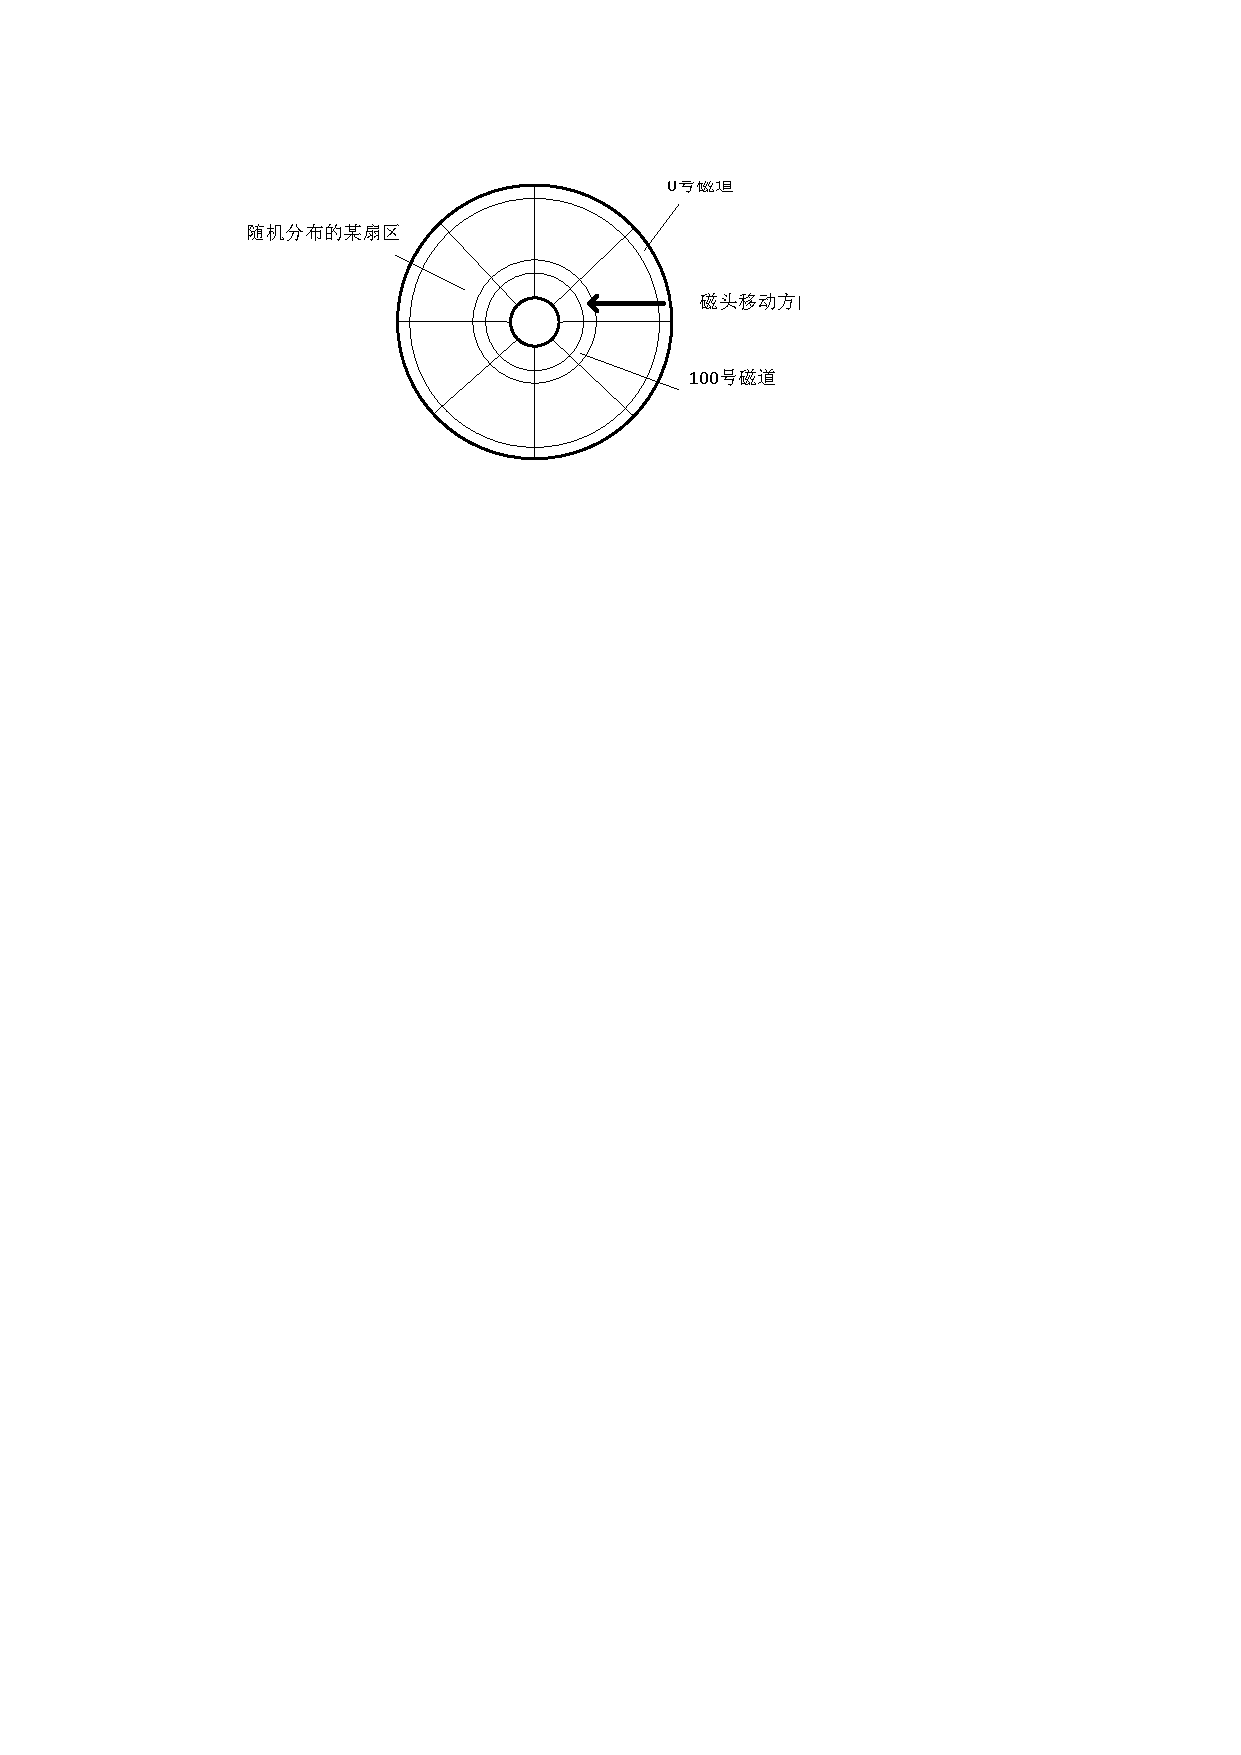
\includegraphics[width=.65\linewidth,height=.4\textheight,keepaspectratio]{../assets/figures/2010-complete-p007-b000.pdf}\end{center}

46. （8 分）设某计算机的逻辑地址空间和物理地址空间均为 64KB，按字节编址。若某进程最多需要 6 页（Page）数据存储空间，页的大小为 1KB，操作系统采用固定分配局部置换策略为此进程分配 4 个页框（Page Frame）。在时刻 260 前的该进程访问情况如下表所示（访问位即使用位）。


\begin{center}\begin{adjustbox}{max width=\linewidth}\begin{tabular}{|>{\raggedright\arraybackslash}p{\dimexpr(\linewidth-8\tabcolsep-5\arrayrulewidth)/4\relax}|>{\raggedright\arraybackslash}p{\dimexpr(\linewidth-8\tabcolsep-5\arrayrulewidth)/4\relax}|>{\raggedright\arraybackslash}p{\dimexpr(\linewidth-8\tabcolsep-5\arrayrulewidth)/4\relax}|>{\raggedright\arraybackslash}p{\dimexpr(\linewidth-8\tabcolsep-5\arrayrulewidth)/4\relax}|}\hline
页号 & 页框号 & 装入时刻 & 访问位\\\hline
0 & 7 & 130 & 1\\\hline
1 & 4 & 230 & 1\\\hline
2 & 2 & 200 & 1\\\hline
3 & 9 & 160 & 1\\\hline\end{tabular}\end{adjustbox}\end{center}

当该进程执行到时刻 260 时，要访问逻辑地址为 17CAH 的数据。请回答下列问题：（1）该逻辑地址对应的页号是多少？（2）若采用先进先出（FIFO）置换算法，该逻辑地址对应的物理地址是多少？要求给出计算过程。（3）若采用时钟（CLOCK）置换算法，该逻辑地址对应的物理地址是多少？要求给出计算过程（设搜索下一页的指针沿顺时针方向移动，且当前指向 2 号页框，示意图如下）。


\begin{center}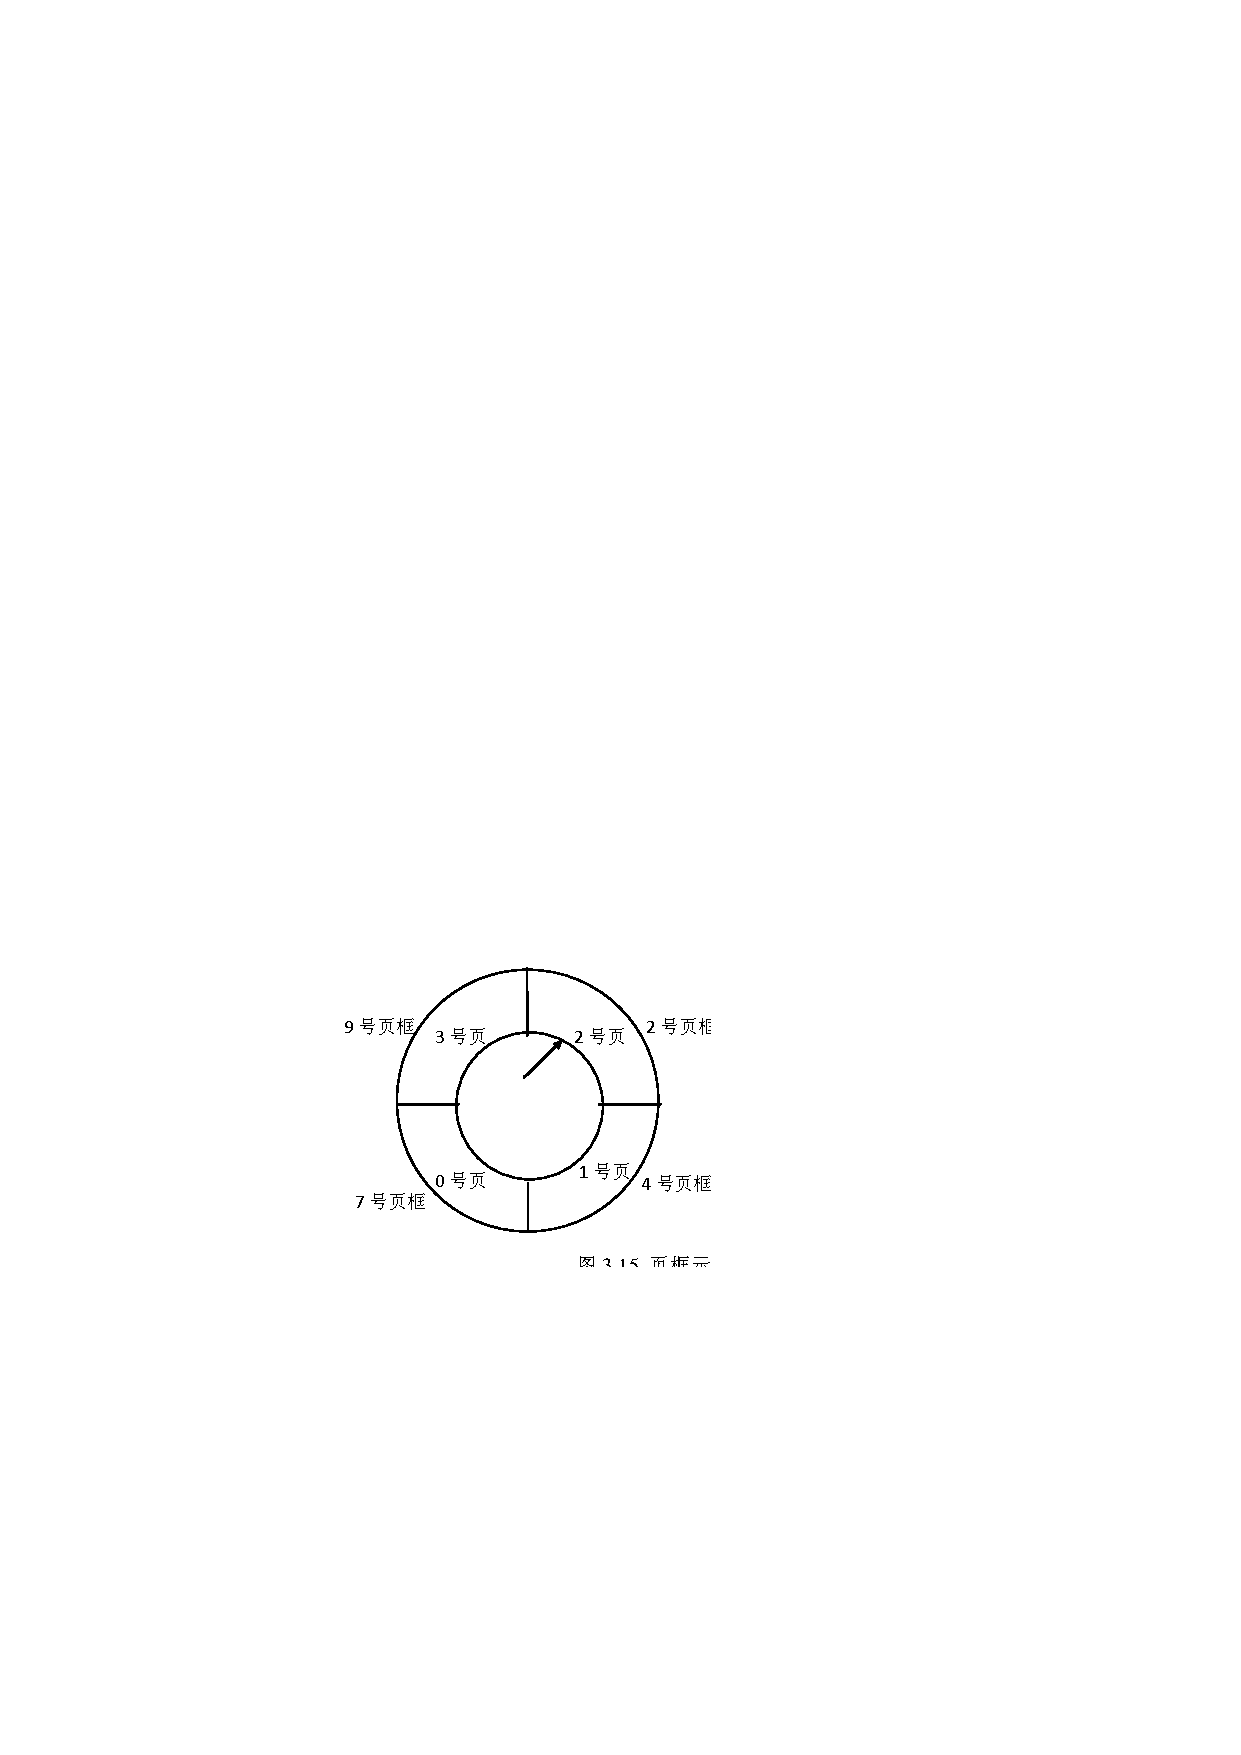
\includegraphics[width=.65\linewidth,height=.4\textheight,keepaspectratio]{../assets/figures/2010-complete-p007-b004.pdf}\end{center}

47. （9 分）某局域网采用CSMA/CD 协议实现介质访问控制，数据传输速率为10Mbps，主机甲和主机乙之间的距离为2 km，信号传播速度是200 000 km/s。请回答下列问题，要求说明理由或写出计算过程。⑴若主机甲和主机乙发送数据时发生冲突，则从开始发送数据时刻起，到两台主机均检测到冲突时刻止，最短需经过多长时间？最长需经过多长时间（假设主机甲和主机乙发送数据过程中，其他主机不发送数据）？⑵若网络不存在任何冲突与差错，主机甲总是以标准的最长以太网数据帧（1 518 字节）向主机乙发送数据，主机乙每成功收到一个数据帧后立即向主机甲发送一个64 字节的确认帧，主机甲收到确认帧后方可发送下一个数据帧。此时主机甲的有效数据传输速率是多少（不考虑以太网的前导码）？


\subsection*{参考答案}

\subsection*{一、单项选择题（后附有解析）}

1. D 2. C 3. D 4. C 5. B 6. A 7. C 8. B


9. B 10. D 11. A 12. D 13. B 14. B 15. D 16. A


17. D 18. B 19. A 20. D 21. A 22. D 23. A 24. C


25. B 26. A 27. D 28. B 29. B 30. C 31. C 32. B


33. C 34. C 35. D 36. C 37. B 38. D 39. A 40. A


\subsection*{二、综合应用题}

41．解答：（1）由装载因子 0.7，数据总数为 7，得一维数组大小为 7/0.7=10，数组下标为 0～9。所构造的散列函数值如下所示：


\begin{center}\begin{adjustbox}{max width=\linewidth}\begin{tabular}{|>{\raggedright\arraybackslash}p{\dimexpr(\linewidth-16\tabcolsep-9\arrayrulewidth)/8\relax}|>{\raggedright\arraybackslash}p{\dimexpr(\linewidth-16\tabcolsep-9\arrayrulewidth)/8\relax}|>{\raggedright\arraybackslash}p{\dimexpr(\linewidth-16\tabcolsep-9\arrayrulewidth)/8\relax}|>{\raggedright\arraybackslash}p{\dimexpr(\linewidth-16\tabcolsep-9\arrayrulewidth)/8\relax}|>{\raggedright\arraybackslash}p{\dimexpr(\linewidth-16\tabcolsep-9\arrayrulewidth)/8\relax}|>{\raggedright\arraybackslash}p{\dimexpr(\linewidth-16\tabcolsep-9\arrayrulewidth)/8\relax}|>{\raggedright\arraybackslash}p{\dimexpr(\linewidth-16\tabcolsep-9\arrayrulewidth)/8\relax}|>{\raggedright\arraybackslash}p{\dimexpr(\linewidth-16\tabcolsep-9\arrayrulewidth)/8\relax}|}\hline
key & 7 & 8 & 30 & 11 & 18 & 9 & 14\\\hline
H(key) & 0 & 3 & 6 & 5 & 5 & 6 & 0\\\hline\end{tabular}\end{adjustbox}\end{center}

采用线性探测再散列法处理冲突，所构造的散列表为：


\begin{center}\begin{adjustbox}{max width=\linewidth}\begin{tabular}{|c|c|c|c|c|c|c|c|c|c|c|}\hline
地址 & 0 & 1 & 2 & 3 & 4 & 5 & 6 & 7 & 8 & 9\\\hline
关键字 & 7 & 14 &  & 8 &  & 11 & 30 & 18 & 9 & \\\hline\end{tabular}\end{adjustbox}\end{center}

（2）查找成功时，是根据每个元素查找次数来计算平均长度，在等概率的情况下，各关键字的查找次数为：


\begin{center}\begin{adjustbox}{max width=\linewidth}\begin{tabular}{|>{\raggedright\arraybackslash}p{\dimexpr(\linewidth-16\tabcolsep-9\arrayrulewidth)/8\relax}|>{\raggedright\arraybackslash}p{\dimexpr(\linewidth-16\tabcolsep-9\arrayrulewidth)/8\relax}|>{\raggedright\arraybackslash}p{\dimexpr(\linewidth-16\tabcolsep-9\arrayrulewidth)/8\relax}|>{\raggedright\arraybackslash}p{\dimexpr(\linewidth-16\tabcolsep-9\arrayrulewidth)/8\relax}|>{\raggedright\arraybackslash}p{\dimexpr(\linewidth-16\tabcolsep-9\arrayrulewidth)/8\relax}|>{\raggedright\arraybackslash}p{\dimexpr(\linewidth-16\tabcolsep-9\arrayrulewidth)/8\relax}|>{\raggedright\arraybackslash}p{\dimexpr(\linewidth-16\tabcolsep-9\arrayrulewidth)/8\relax}|>{\raggedright\arraybackslash}p{\dimexpr(\linewidth-16\tabcolsep-9\arrayrulewidth)/8\relax}|}\hline
key & 7 & 8 & 30 & 11 & 18 & 9 & 14\\\hline
次数 & 1 & 1 & 1 & 1 & 3 & 3 & 2\\\hline\end{tabular}\end{adjustbox}\end{center}

故，\(\displaystyle ASL_{\text{成功}}=(1+2+1+1+1+3+3)/7=12/7\)。这里要特别防止惯性思维。查找失败时，是根据查找失败位置计算平均次数，根据散列函数 MOD 7，初始只可能在 0～6 的位置。等概率情况下，查找 0～6 位置查找失败的查找次数为：


\begin{center}\begin{adjustbox}{max width=\linewidth}\begin{tabular}{|>{\raggedright\arraybackslash}p{\dimexpr(\linewidth-16\tabcolsep-9\arrayrulewidth)/8\relax}|>{\raggedright\arraybackslash}p{\dimexpr(\linewidth-16\tabcolsep-9\arrayrulewidth)/8\relax}|>{\raggedright\arraybackslash}p{\dimexpr(\linewidth-16\tabcolsep-9\arrayrulewidth)/8\relax}|>{\raggedright\arraybackslash}p{\dimexpr(\linewidth-16\tabcolsep-9\arrayrulewidth)/8\relax}|>{\raggedright\arraybackslash}p{\dimexpr(\linewidth-16\tabcolsep-9\arrayrulewidth)/8\relax}|>{\raggedright\arraybackslash}p{\dimexpr(\linewidth-16\tabcolsep-9\arrayrulewidth)/8\relax}|>{\raggedright\arraybackslash}p{\dimexpr(\linewidth-16\tabcolsep-9\arrayrulewidth)/8\relax}|>{\raggedright\arraybackslash}p{\dimexpr(\linewidth-16\tabcolsep-9\arrayrulewidth)/8\relax}|}\hline
H(key) & 0 & 1 & 2 & 3 & 4 & 5 & 6\\\hline
次数 & 3 & 2 & 1 & 2 & 1 & 5 & 4\\\hline\end{tabular}\end{adjustbox}\end{center}

故，\(\displaystyle ASL_{\text{不成功}}=(3+2+1+2+1+5+4)/7=18/7\)。


42．解答：（1）算法的基本设计思想：可以将这个问题看做是把数组 ab 转换成数组 ba（a 代表数组的前 p 个元素，b 代表数组中余下的 n-p 个元素），先将 a 逆置得到 \(\displaystyle a^{-1}b\)，再将 b 逆置得到 \(\displaystyle a^{-1}b^{-1}\)，最后将整个 \(\displaystyle a^{-1}b^{-1}\) 逆置得到\(\displaystyle (a^{-1}b^{-1})^{-1}=ba\)。设 Reverse 函数执行将数组元素逆置的操作，对 abcdefgh 向左循环移动 3（p=3）个位置的过程如下：Reverse(0,p-1) 得到 cbadefgh；Reverse(p,n-1) 得到 cbahgfed；Reverse(0,n-1) 得到 defghabc；注：Reverse 中，两个参数分别表示数组中待转换元素的始末位置。（2）使用 c 语言描述算法如下：


\begin{Verbatim}[breaklines,breakanywhere,fontsize=\small]
void Reverse(int R[], int from, int to) {
    int i, temp;
    for (i = 0; i < (to-from+1)/2; i++)
\end{Verbatim}

\begin{Verbatim}[breaklines,breakanywhere,fontsize=\small]
{
    temp = R[from+i];
    R[from+i] = R[to-i];
    R[to-i] = temp;
}
} // Reverse
void Converse(int R[], int n, int p) {
    Reverse(R,0,p-1);
    Reverse(R,p,n-1);
    Reverse(R,0,n-1);
}
\end{Verbatim}

（3）上述算法中三个 Reverse 函数的时间复杂度分别为 \(\displaystyle O(p/2)\)、\(\displaystyle O((n-p)/2)\) 和 \(\displaystyle O(n/2)\)，故所设计算法的时间复杂度为 \(\displaystyle O(n)\)，空间复杂度为 \(\displaystyle O(1)\)。另解，借助辅助数组来实现：算法思想：创建大小为 p 的辅助数组 S，将 R 中前 p 个整数依次暂存在 S 中，同时将 R 中后 n-p 个整数左移，然后将 S 中暂存的 p 个数依次放回到 R 中的后续单元。时间复杂度为 \(\displaystyle O(n)\)，空间复杂度为 \(\displaystyle O(p)\)。


43．解答：(1) 操作码占4 位，则该指令系统最多可有\(\displaystyle 2^4=16\) 条指令；操作数占6 位，寻址方式占3 位，于是寄存器编号占3 位，则该机最多有\(\displaystyle 2^3=8\) 个通用寄存器；主存容量128KB，按字编址，计算机字长为16 位，划分为128KB/2B=\(\displaystyle 2^{16}\) 个存储单元，故MDR 和MAR 至少各需16 位。(2) PC 和Rn 可表示的地址范围均为0～\(\displaystyle 2^{16}\)-1，而主存地址空间为\(\displaystyle 2^{16}\)，故转移指令的目标地址范围是0000H～FFFFH（0～\(\displaystyle 2^{16}\)-1）。(3) 汇编语句“add (R4), (R5) +”，对应的机器码为0010 0011 0001 0101B=2315H。该指令执行后，寄存器R5 和存储单元5678H 的内容会改变。执行后，R5 的内容从5678H 变成5679H。存储单元5678H 中的内容变成该加法指令计算的结果5678H＋1234H=68ACH。


44．解答：(1) 数据Cache 有8 个Cache 行，每个Cache 行大小为64B，Cache 中每个字块的Tag 字段的位数是\(\displaystyle 28-9=19\) 位，此外还需使用一个有效位，合计20 位。因此，数据Cache 的总容量应为：\(\displaystyle 8\times(64+20/8)\mathrm{B}=532\mathrm{B}\)。(2) 数组a 在主存的存放位置及其与Cache 之间的映射关系如下图所示：数组按行优先方式存放，首地址为320，数组元素占四个字节。a[0][31]所在的主存块对应的Cache 行号为：(320＋31×4) DIV 64 = 6 ；a[1][1]所在的主存块对应的Cache 行号为：(320＋256×4＋1×4) DIV 64 MOD 8 = 5 。(3) 编译时i、j、sum 均分配在寄存器中，故数据访问命中率仅考虑数组a 的情况。\textcircled{1}该程序的特点是数组中的每一个元素仅被使用一次。数组a 按行优先存放，数据Cache 正好放下数组半行中的全部元素，即元素的存储顺序与使用次序高度的吻合，每个字块的16 个int 型元素中，除访问的第一个不会命中，接下来的15 个都会命中。访问全部字块都符合这一规律，故命中率为15／16，即程序A 的数据访问命中率是93.75\%。\textcircled{2}程序B 按照数组的列执行外层循环，在执行内层循环的过程中，将连续访问不同行的同一列的数据，不同行的同一列数组使用的是同一个Cache 单元，每次都不会命中，故命中率是0由于从Cache 读数据比从主存读数据快很多，所以程序A 的执行比程序B 快得多。注意：本题考查Cache 容量计算，直接映射方式的地址计算，以及命中率计算（注意：行优先遍历与列优先遍历命中率差别很大）。


\begin{center}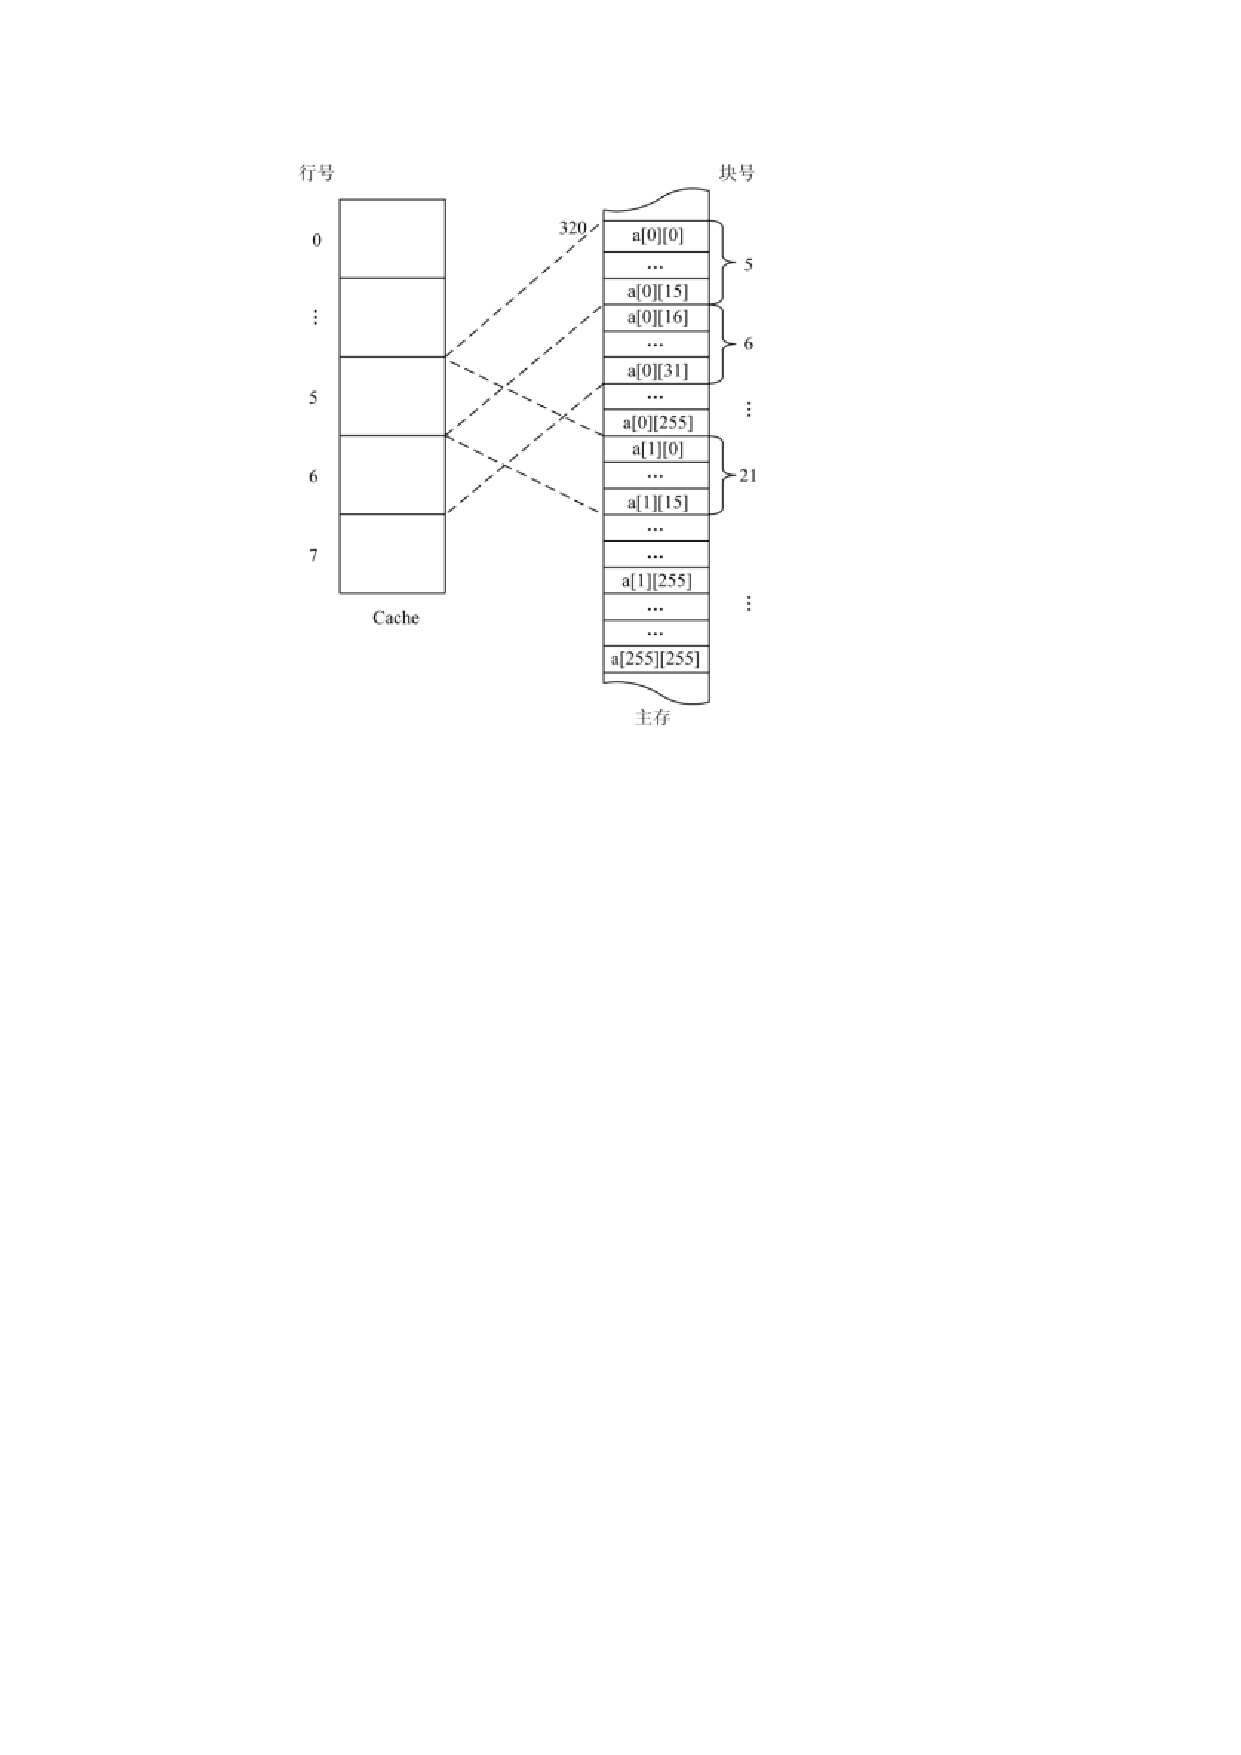
\includegraphics[width=.65\linewidth,height=.4\textheight,keepaspectratio]{../assets/figures/2010-complete-p010-b000.pdf}\end{center}

45．解答：（1）用位图表示磁盘的空闲状态。每一位表示一个磁盘块的空闲状态，共需要 16 384/32=512 个字=512×4 个字节=2KB，正好可放在系统提供的内存中。（2）采用 CSCAN 调度算法，访问磁道的顺序和移动的磁道数如下表所示：


\begin{center}\begin{adjustbox}{max width=\linewidth}\begin{tabular}{|>{\raggedright\arraybackslash}p{\dimexpr(\linewidth-4\tabcolsep-3\arrayrulewidth)/2\relax}|>{\raggedright\arraybackslash}p{\dimexpr(\linewidth-4\tabcolsep-3\arrayrulewidth)/2\relax}|}\hline
被访问的下一个磁道号 & 移动距离（磁道数）\\\hline
120 & 20\\\hline
30 & 90\\\hline
50 & 20\\\hline
90 & 40\\\hline\end{tabular}\end{adjustbox}\end{center}

移动的磁道数为 20+90+20+40=170，故总的移动磁道时间为 170ms。由于转速为 6000r/m，则平均旋转延迟为 5ms，总的旋转延迟时间=20ms。由于转速为 6000r/m，则读取一个磁道上一个扇区的平均读取时间为 0.1ms，总的读取扇区的时间为 0.4ms。综上，读取上述磁道上所有扇区所花的总时间为 190.4ms。（3）采用 FCFS（先来先服务）调度策略更高效。因为 Flash 半导体存储器的物理结构不需要考虑寻道时间和旋转延迟，可直接按 I/O 请求的先后顺序服务。


46．解答：（1）由于该计算机的逻辑地址空间和物理地址空间均为 \(\displaystyle 64\mathrm{KB}=2^{16}\mathrm{B}\)，按字节编址，且页的大小为 \(\displaystyle 1\mathrm{K}=2^{10}\)，故逻辑地址和物理地址的地址格式均为：


\begin{center}\begin{adjustbox}{max width=\linewidth}\begin{tabular}{|>{\raggedright\arraybackslash}p{\dimexpr(\linewidth-4\tabcolsep-3\arrayrulewidth)/2\relax}|>{\raggedright\arraybackslash}p{\dimexpr(\linewidth-4\tabcolsep-3\arrayrulewidth)/2\relax}|}\hline
页号/页框号（6 位） & 页内偏移量（10 位）\\\hline\end{tabular}\end{adjustbox}\end{center}

17CAH = 0001 0111 1100 1010B，可知该逻辑地址的页号为 000101B = 5。（2）根据 FIFO 算法，需要替换装入时间最早的页，故需要置换装入时间最早的 0 号页，即将 5 号页装入 7 号页框中，所以物理地址为 0001 1111 1100 1010B = 1FCAH。（3）根据 CLOCK 算法，如果当前指针所指页框的使用位为 0，则替换该页；否则将使用位清零，并将指针指向下一个页框，继续查找。根据题设和示意图，将从 2 号页框开始，前 4 次查找页框号的顺序为


2→4→7→9，并将对应页框的使用位清零。在第5 次查找中，指针指向2 号页框，因2 号页框的使用位为0，故淘汰2 号页框对应的2 号页，把5 号页装入2 号页框中，并将对应使用位设置为1，所以对应的物理地址为0000 1011 1100 1010B = 0BCAH。


47．解答：⑴当主机甲和主机乙同时向对方发送数据时，信号在信道中发生冲突后，冲突信号继续向两个方向传播。这种情况下两台主机均检测到冲突需要经过的时间最短，等于单程的传播时延 t0= 2km/200 000km/s =


0.01ms 。主机甲（或主机乙）先发送一个数据帧，当该数据帧即将到达主机乙（或主机乙）时，主机乙（或主机甲）也开始发送一个数据帧，这时，主机乙（或主机甲）将立刻检测到冲突，而主机甲（或主机乙）要检测到冲突，冲突信号还需要从主机乙（或主机甲）传播到主机甲（或主机乙），因此甲乙两台主机均检测到冲突所需的最长时间等于双程的传播时延 2*t0 = 0.02ms 。⑵主机甲发送一个数据帧的时间，即发送时延 t1 = 1518×8b/10Mbps = 1.2144 ms ；主机乙每成功收到一个数据帧后，向主机甲发送确认帧，确认帧的发送时延 t2 = 64×8b/10Mbps = 0.0512ms ；主机甲收到确认帧后，即发送下一数据帧，故主机甲的发送周期T = 数据帧发送时延 t1 + 确认帧发送时延 t2 + 双程传播时延= t1 + t2 + 2*t0 = 1.2856 ms ；于是主机甲的有效数据传输率为1500×8/T = 12000b/1.2856 ms ≈ 9.33 Mbps。（以太网有效数据1500 字节，即以太网帧的数据部分）


\subsection*{2010 年全国硕士研究生入学统一考试计算机学科专业基础综合试题——选择题部分解析}

\subsection*{一、单项选择题}

1．考查限定条件的出栈序列。A 可由in,in,in,in,out,out,in,out,out,in,out,out 得到；B 可由in,in,in,out,out,in,out,out,in,out,in,out 得到；C 可由in,in,out,in,out,out,in,in,out,in,out,out 得到；D 可由in,out,in,in,in,in,in,out,out,out,out,out 得到，但题意要求不允许连续三次退栈操作，故D 错。


2．考查受限的双端队列的出队序列。A 可由左入，左入，右入，右入，右入得到 B 可由 左入，左入，右入，左入，右入得到。D 可由左入，左入，左入，右入，左入得到 所以不可能得到C。


3．考查线索二叉树的基本概念和构造。题中所给二叉树的后序序列为dbca 。结点d 无前驱和左子树，左链域空，无右子树，右链域指向其后继结点b；结点b 无左子树，左链域指向其前驱结点d；结点c 无左子树，左链域指向其前驱结点b，无右子树，右链域指向其后继结点a。


4．考查平衡二叉树的插入算法。插入48 以后，该二叉树根结点的平衡因子由-1 变为-2，失去平衡，需进行两次旋转（先右旋后左旋）操作。


5．考查树结点数的特性。设树中度为 \(\displaystyle i\,(i=0,\allowbreak 1,\allowbreak 2,\allowbreak 3,\allowbreak 4)\) 的结点数分别为 \(\displaystyle N_i\)，树中结点总数为 \(\displaystyle N\)，则树中各结点的度之和等于 \(\displaystyle N-1\)，即 \(\displaystyle N=1+N_1+2N_2+3N_3+4N_4=N_0+N_1+N_2+N_3+N_4\)。根据题设中的数据，即可得到 \(\displaystyle N_0=82\)，即树 T 的叶结点的个数是 82。


6．考查哈弗曼树的特性。哈夫曼树为带权路径长度最小的二叉树，不一定是完全二叉树。哈夫曼树中没有度为１的结点，B 正确；构造哈夫曼树时，最先选取两个权值最小的结点作为左右子树构造一棵新的二叉树，C 正确；哈夫曼树中任一非叶结点P 的权值为其左右子树根结点权值之和，其权值不小于其左右子树根结点的权值，在与结点P 的左右子树根结点处于同一层的结点中，若存在权值大于结点P 权值的结点Q，那么结点Q的兄弟结点中权值较小的一个应该与结点P 作为左右子树构造新的二叉树，综上可知，哈夫曼树中任一非叶结点的权值一定不小于下一层任一结点的权值。


7．考查图的连通性。要保证无向图G 在任何情况下都是连通的，即任意变动图G 中的边，G 始终保持连通，首先需要G的任意六个结点构成完全连通子图G1，需15 条边，然后再添一条边将第7 个结点与G1 连接起来，共需16 条边。


8．考查拓扑排序序列。题中图有三个不同的拓扑排序序列，分别为 abced，abecd，aebcd。


9．考查折半查找的过程。具有 \(\displaystyle n\) 个结点的判定树的高度为 \(\displaystyle \lfloor\log_2n\rfloor+1\)，长度为 16，高度为 5，所以最多比较 5 次。


10．考查快速排序。


递归次数与各元素的初始排列有关。如果每一次划分后分区比较平衡，则递归次数少，如果划分后分区不平衡，则递归次数多。递归次数与处理顺序无关。


11．考查各种排序算法的过程。看第一趟可知仅有88 被移到最后.如果是希尔排序，则12，88，10 应变为10，12，88。因此排除希尔排序。如果是归并排序，则应长度为2 的子序列是有序的，由此可排除归并。如果是基数排序，则16，5，10 应变为10，5，16，由此排除基数。可以看到，每一趟都有一个元素移到其最终位置，符合冒泡排序特点。


12．考查计算机的性能指标。Ⅰ.CPU 的时钟频率，也就是CPU 主频率，一般说来，一个时钟周期内完成的指令数是固定的，所以主频越高，CPU 的速度也就快，程序的执行时间就越短。Ⅱ.数据在功能部件之间传送的路径称为数据通路，数据通路的功能是实现CPU 内部的运算器和寄存器以及寄存器之间的数据交换。优化数据通路结构，可以有效提高计算机系统的吞吐量，从而加快程序的执行。Ⅲ.计算机程序需要先转化成机器指令序列才能最终得到执行，通过对程序进行编译优化可以得到更优的指令序列，从而使得程序的执行时间也越短。


13．考查定点数的运算。用补码表示时8 位寄存器所能表示的整数范围为-128\textasciitilde{}+127。由于r1 = -2，r2 = -14，r3 = -112，r4 = -8，则r2×r3 = 1568，结果溢出。


14．考查不同精度的数在计算机中的表示方法及其相互装换。由于（int）f=1，小数点后面4 位丢失，故II 错。IV 的计算过程是先将f 转化为双精度浮点数据格式，然后进行加法运算，故（d+f）-d 得到的结果为双精度浮点数据格式，而f 为单精度浮点数据格式，故IV错。


15．考查存储器的组成和设计。用 \(\displaystyle 2\mathrm{K}\times4\) 位的芯片组成一个 \(\displaystyle 8\mathrm{K}\times8\) 位存储器，每行中所需芯片数为 2，每列中所需芯片数为 4，各行芯片的地址分配为：


\begin{center}\begin{adjustbox}{max width=\linewidth}\begin{tabular}{|>{\raggedright\arraybackslash}p{\dimexpr(\linewidth-4\tabcolsep-3\arrayrulewidth)/2\relax}|>{\raggedright\arraybackslash}p{\dimexpr(\linewidth-4\tabcolsep-3\arrayrulewidth)/2\relax}|}\hline
芯片行 & 地址范围\\\hline
第一行（2 个芯片并联） & 0000H～07FFH\\\hline
第二行（2 个芯片并联） & 0800H～0FFFH\\\hline
第三行（2 个芯片并联） & 1000H～17FFH\\\hline
第四行（2 个芯片并联） & 1800H～1FFFH\\\hline\end{tabular}\end{adjustbox}\end{center}

于是地址 0B1FH 所在芯片的最小地址即为 0800H。


16．考查半导体随机存取存储器。一般Cache 采用高速的SRAM 制作，比ROM 速度快很多，因此III 是错误的，排除法即可选A。RAM 需要刷新，而ROM 不需要刷新。


17．考查TLB、Cache 及Page 之间的关系。TLB 即为快表，快表只是慢表（Page）的小小副本，因此TLB 命中，必然Page 也命中，而当Page命中，TLB 则未必命中，故D 不可能发生；而Cache 的命中与否与TLB、Page 的命中与否并无必然联系。


18．考查CPU 内部寄存器的特性。汇编程序员可以通过指定待执行指令的地址来设置PC 的值，而IR，MAR，MDR 是CPU 的内部工作寄存器，对程序员不可见。


19．考查指令流水线的基本概念。有三种相关可能引起指令流水线阻塞：1. 结构相关，又称资源相关；2. 数据相关；3. 控制相关，主要由转移指令引起。数据旁路技术，其主要思想是不必待某条指令的执行结果送回到寄存器，再从寄存器中取出该结果，作为下一条指令的源操作数，而是直接将执行结果送到其他指令所需要的地方，这样可以使流水线不发生停顿。


20．考查典型的总线标准，目前典型的总线标准有：ISA、EISA、VESA、 PCI 、PCI-Express、AGP、USB、RS-232C 等。


21．考查中断处理过程。单级中断系统中，不允许中断嵌套。中断的处理过程为：1. 关中断；2. 保存断点；3. 识别中断源；4. 保存现场；5. 中断事件处理；（开中断、执行中断服务程序、关中断）6. 恢复现场；7. 开中断；8. 中断返回。其中，1\textasciitilde{}3 步由硬件完成，4\textasciitilde{}8 由中断服务程序完成。


22．考查显示器相关概念。刷新所需带宽 = 分辨率×色深×帧频 = 1600×1200×24b×85HZ = 3916.8Mbps，显存总带宽的50\%用来刷屏，于是需要的显存总带宽为3916.8/0.5 = 7833.6Mbps ≈ 7834Mbps。


23．考查操作系统的接口。系统调用是能完成特定功能的子程序，当应用程序要求操作系统提供某种服务时，便调用具有相应功能的系统调用。库函数则是高级语言中提供的与系统调用对应的函数（也有些库函数与系统调用无关），目的是隐藏访管指令的细节，使系统调用更为方便抽象。但要注意，库函数属于用户程序而非系统调用，是系统调用的上层。


24．考查引起创建进程的事件。引起进程创建的事件有：用户登录、作业调度、提供服务、应用请求等，本题的选项分别对应：Ⅰ用户登录成功 在分时系统中，用户登录成功，系统将为终端建立一个进程。Ⅱ设备分配 设备分配是通过在系统中设置相应的数据结构实现的，不需要创建进程。Ⅲ启动程序执行 典型的引起创建进程的事件。


25．考查信号量的原理。信号量表示当前的可用相关资源数。当信号量K>0 时，表示还有K 个相关资源可用；而当信号量K<0 时，表示有|K|个进程在等待该资源。所以该资源可用数是1，等待该资源的进程数是0。


26．考查进程调度。进程时间片用完，从执行态进入就绪态应降低优先级以让别的进程被调度进入执行状态。B 中进程刚完成I/O，进入就绪队列后应该等待被处理机调度，故应提高优先权；C 中有类似的情况；D 中不应该在此时降低，应该在时间片用完后降低。


27．考查进程间通信与Peterson 算法。此算法实现互斥的主要思想在于设置了一个turn 变量，用于进程间的互相“谦让”。一般情况下，如果进程p0 试图访问临界资源，设置flag[0]=true，表示希望访问。此时如果进程p1还未试图访问临界资源，则flag[1]在进程上一次访问完临界资源退出临界区后已设置为false。所以进程p0 在执行循环判断条件时，第一个条件不满足，进程p0 可以正常进入临界区，且满足互斥条件。我们需要考虑的是两个进程同时试图访问临界资源的情况。注意turn 变量的含义：进程在试图访问时，首先设置自己的flag 变量为true，表示希望访问；但又设置turn 变量为对方的进程编号，表示“谦让”，因为在循环判断条件中turn 变量不是自己编号时就循环等待。这时两个进程就会互相“谦让”一番，但是这不会造成饥饿的局面，因为turn 变量会有一个最终值，所以必定有进程可以结束循环进入临界区。实际的情况是，先作出“谦让”的进程先进入临界区，后作出“谦让”的进程则需要循环等待。


其实这里可以想象为两个人进门，每个人进门前都会和对方客套一句“你走先”。如果进门时没别人，就当和空气说句废话，然后大步登门入室；如果两人同时进门，就互相请先，但各自只客套一次，所以先客套的人请完对方，就等着对方请自己，然后光明正大进门。


28．考查动态分区分配。考生需对动态分区分配的四种算法加以理解。最佳适配算法是指：每次为作业分配内存空间时，总是找到能满足空间大小需要的最小的空闲分区给作业。可以产生最小的内存空闲分区。下图显示了这个过程的主存空间的变化：图中，灰色部分为分配出去的空间，白色部分为空闲区。这样，容易发现,此时主存中最大空闲分区的大小为9Mb。


\begin{center}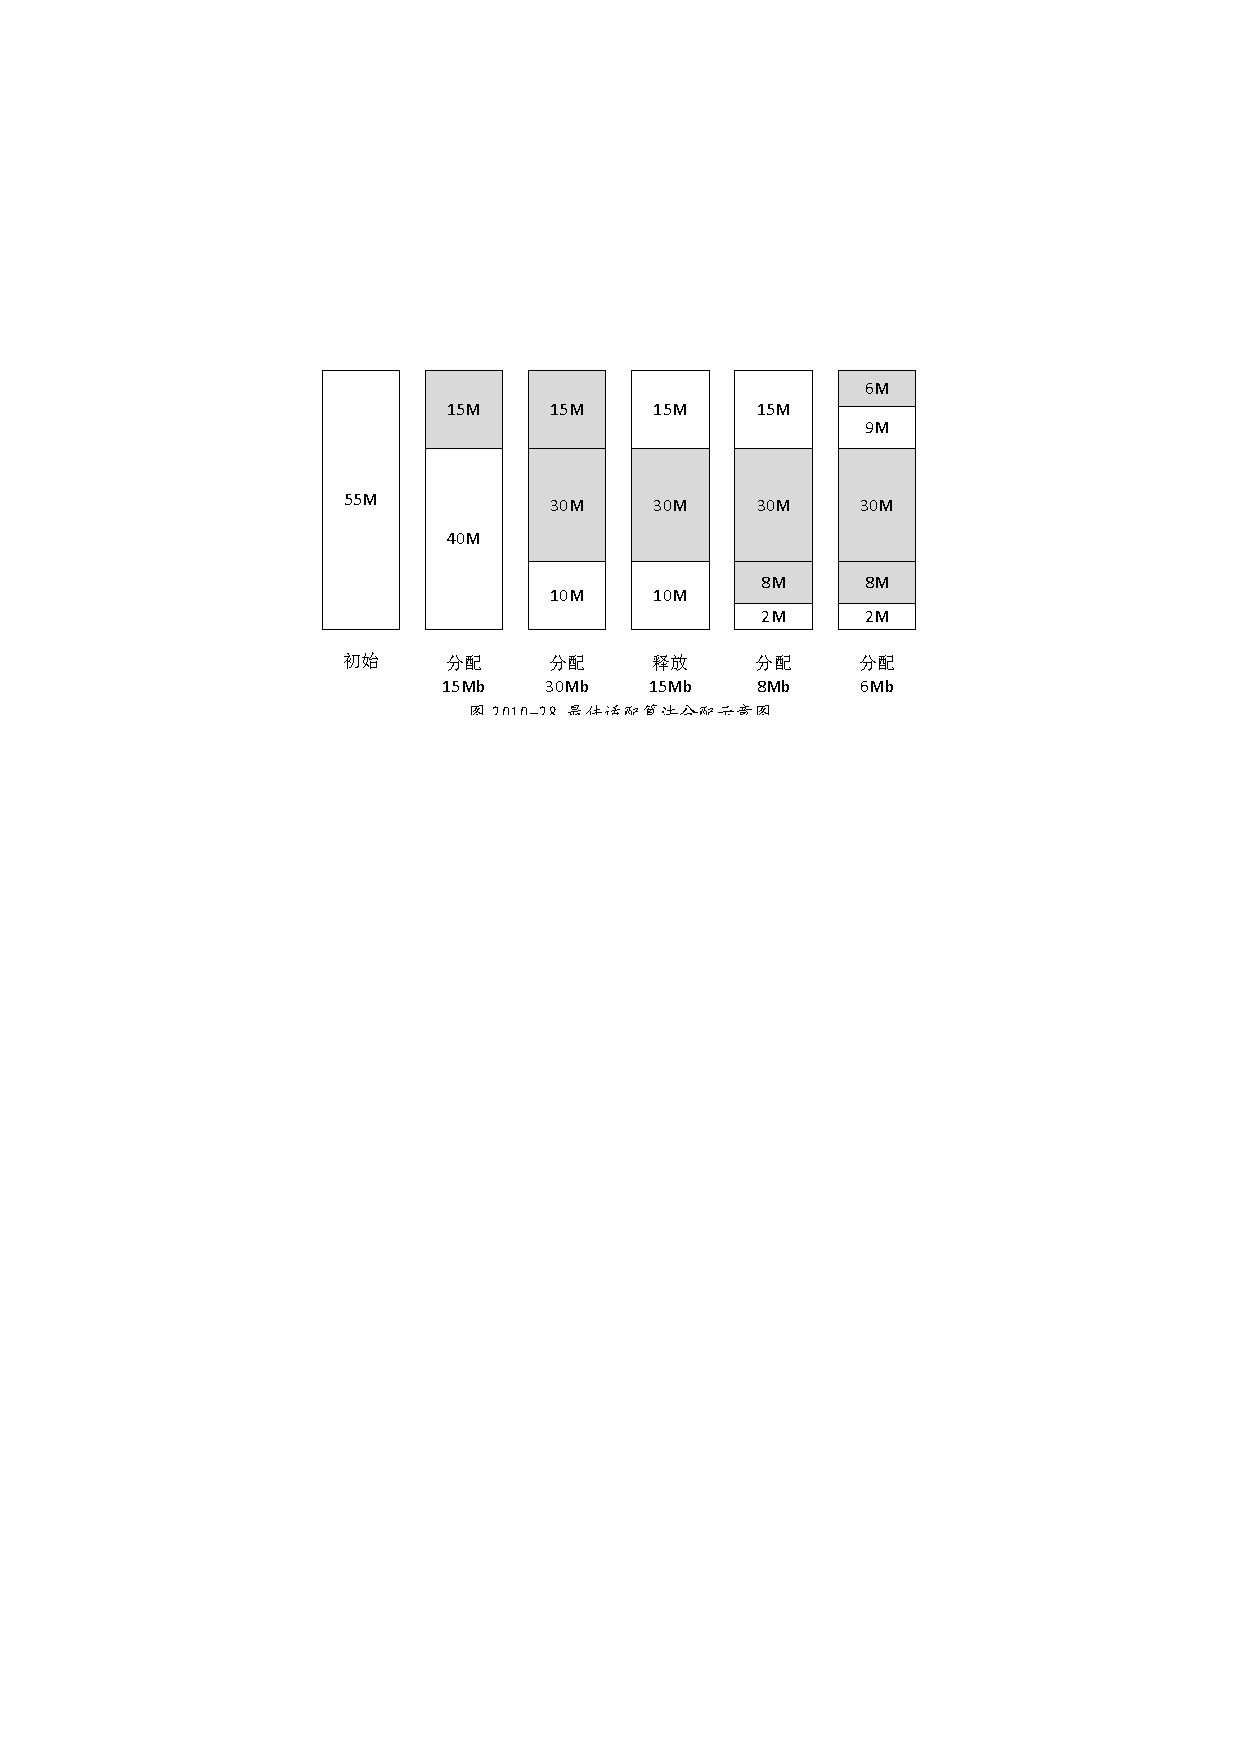
\includegraphics[width=.65\linewidth,height=.4\textheight,keepaspectratio]{../assets/figures/2010-complete-p015-b002.pdf}\end{center}

29．考查非连续分配的分页存储管理方式。页大小为 \(\displaystyle 2^{10}\) 字节，页表项大小为 2 字节，采用二级页表，一页可存放 \(\displaystyle 2^9\) 个页表项，逻辑地址空间大小为 \(\displaystyle 2^{16}\) 页，要使表示整个逻辑地址空间的页目录表中包含的表项个数最少，则需要 \(\displaystyle 2^{16}/2^9=2^7=128\) 个页面保存页表项，即页目录表中包含的个数最少为 128。


30．考查磁盘文件的大小性质。因每个磁盘索引块和磁盘数据块大小均为256 字节。所以4 个直接地址索引指向的数据块大小为4×256 字节。2 个一级间接索引共包括2×(256÷4)个直接地址索引，既其指向的数据块大小为2×(256÷4)×256 字节。1 个二级间接地址索引所包含的直接地址索引数为(256÷4) ×(256÷4)，即其所指向的数据块大小为(256÷4) ×(256÷4) ×256 字节。即7 个地址项所指向的数据块总大小为\(\displaystyle 4\times256+2\times(256/4)\times256+(256/4)^2\times256=1082368\) 字节=1057KB。


31．考查当前目录的作用。一个文件系统含有许多级时，每访问一个文件，都要使用从树根开始直到树叶为止，包括各中间节点名的全路径名。当前目录又称工作目录，进程对各个文件的访问都相对于当前目录进行，所以检索速度要快于检索全路径名。


32．考查中断处理。键盘是典型的通过中断I/O 方式工作的外设，当用户输入信息时，计算机响应中断并通过中断处理程序获得输入信息。


33．考查计算机网络体系结构的基本概念。我们把计算机网络的各层及其协议的集合称为体系结构。因此A、B、D 正确，而体系结构是抽象的，它不包括各层协议及功能的具体实现细节。


34．考查存储转发机制。由题设可知，分组携带的数据长度为980B，文件长度为980000B，需拆分为1000 个分组，加上头


部后，每个分组大小为1000B，总共需要传送的数据量大小为1MB。由于所有链路的数据传输速度相同，因此文件传输经过最短路径时所需时间最少，最短路径经过2 个分组交换机。当t = 1M×8/100Mbps = 80ms 时，H1 发送完最后一个bit；由于传输延时，当H1 发完所有数据后，还有两个分组未到达目的地，其中最后一个分组，需经过2个分组交换机的转发，在两次转发完成后，所有分组均到达目的主机。每次转发的时间为 t0 =1K×8/100Mbps = 0.08ms。所以，在不考虑分组拆装时间和等待延时的情况下，当t = 80ms + 2t0 = 80.16ms 时，H2 接收完文件，即所需的时间至少为80.16ms。


35．考查RIP 路由协议。RIP 使用距离向量算法的工作过程参见内容精讲部分。R1 在收到信息并更新路由表后，若需要经过R2 到达net1，则其跳数为17，由于距离为16 表示不可达，因此R1 不能经过R2 到达net1，R2 也不可能到达net1。B、C 错误，D 正确。而题目中并未给出R1 向R2 发送的信息，因此A 也不正确。


36．考查ICMP 协议。ICMP 差错报告报文有5 种，终点不可达、源点抑制、时间超过、参数问题、改变路由（重定向），其中源点抑制是当路由器或主机由于拥塞而丢弃数据报时，就向源点发送源点抑制报文，使源点知道应当把数据报的发送速率放慢。


37．考查子网划分与子网掩码、CIDR。由于该网络的 IP 地址为 192.168.5.0/24，因此其网络号为前 24 位。第 25—32 位为子网位+主机位。而子网掩码为 255.255.255.248，其第 25—32 位的 248 用二进制表示为 11111000，因此后 8 位中，前 5 位用于子网号，后 3 位用于主机号。RFC 950 文档规定，对分类的 IPv4 地址进行子网划分时，子网号不能为全 1 或全 0。但随着无分类域间路由选择 CIDR 的广泛使用，现在全 1 和全 0 的子网号也可以使用了，但一定要谨慎使用，要弄清你的路由器所有的路由选择软件是否支持全 0 或全 1 的子网号这种用法。但不论是分类的 IPv4 地址还是无分类域间路由选择 CIDR，其子网中的主机号均不能为全 1 或全 0。因此该网络空间的最大子网个数为 \(\displaystyle 2^5=32\) 个，每个子网内的最大可分配地址个数为 \(\displaystyle 2^3-2=6\) 个。


38．考查网络设备与网络风暴。物理层设备中继器和集线器既不隔离冲突域也不隔离广播域；网桥可隔离冲突域，但不隔离广播域；网络层的路由器既隔离冲突域，也隔离广播域；VLAN 即虚拟局域网也可隔离广播域。对于不隔离广播域的设备，他们互连的不同网络都属于同一个广播域，因此扩大了广播域的范围，更容易产生网络风暴。


39．考查TCP 流量控制与拥塞控制。发送方的发送窗口的上限值应该取接收方窗口和拥塞窗口这两个值中较小的一个，于是此时发送方的发送窗口为MIN\{4000，2000\}=2000 字节，由于发送方还没有收到第二个最大段的确认，所以此时主机甲还可以向主机乙发送的最大字节数为2000-1000=1000 字节。


40．考查DNS 系统域名解析过程。当采用递归查询的方法解析域名时，如果主机所询问的本地域名服务器不知道被查询域名的 IP 地址，那么本地域名服务器就以 DNS 客户的身份，向其他根域名服务器继续发出查询请求报文，这种方法用户主机和本地域名服务器发送的域名请求条数均为1 条。

\end{document}
